\newcommand{\mypapersize}{A4}
%% e.g., "A4", "letter", "legal", "executive", ...
%% The size of the paper of the resulting PDF file.

\newcommand{\mylaterality}{oneside} %TODO: change to twoside when finished
%% "oneside" or "twoside"
%% Either you are creating a document which is printed on both, left pages
%% and right pages (twoside) or you create a document which is printed
%% on right pages only (oneside).

\newcommand{\mydraft}{true}
%% "true" or "false"
%% Use draft mode? If true, included graphics are replaced by empty
%% rectangles (of same size) and overfull boxes (in margin space) are
%% marked with black box (-> easy to spot!)

\newcommand{\myparskip}{full}
%% e.g., "no", "full", "half", ...
%% How to separate paragraphs: indention ("no") or spacing ("half",
%% "full", ...).

\newcommand{\myBCOR}{0mm}
%% Inner binding correction. This value depends on the method which is
%% being used to bind your printed result. Some techniques do not
%% require a binding correction at all ("0mm"), other require for
%% example "5mm". Refer to KOMA script documentation for a detailed
%% explanation what a binding correction is and how to measure it.

\newcommand{\myfontsize}{12pt}

\newcommand{\mylinespread}{1.0}

\newcommand{\mylanguage}{ngerman,american}
%% NOTE: The *last* language is the active one!
%% See babel documentation for further details.

%% BibLaTeX-settings: (see biblatex reference for further description)
\newcommand{\mybiblatexstyle}{alphabetic}

\newcommand{\mybiblatexdashed}{false}  %% "true" or "false"
%% If true: replace recurring reference authors with a dash.

\newcommand{\mybiblatexbackref}{true}  %% "true" or "false"
%% If true: create backward links from reference to citations.

\newcommand{\mybiblatexfile}{references-biblatex.bib}
%% Name of the biblatex file that holds the references.

\newcommand{\mydispositioncolor}{0,0,0}
%% e.g., "30,103,182" (blue/turquois), "0,0,0" (black), ...
%% Color of the headings and so forth in RGB (red,green,blue) values.
%% NOTE: if you are using "0,0,0" for black, printers might still
%%       recognize pages as color pages. In case this is a problem
%%       (paying for color print-outs vs. paying for b/w-printouts)
%%       please edit file "template/preamble.tex" and change
%%       "\definecolor{DispositionColor}{RGB}{\mydispositioncolor}"
%%       to "\definecolor{DispositionColor}{gray}{0}" and thus
%%       overwriting the value of \mydispositioncolor above.

\newcommand{\mycolorlinks}{true}  %% "true" or "false"
%% Enables or disables colored links (hyperref package).

\newcommand{\mytitlepage}{template/title_Thesis_TU_Graz}

\newcommand{\mytodonotesoptions}{}
%% e.g., "" (empty), "disable", ...
%% Options for the todonotes-package. If "disable", all todonotes will
%% be hidden (including listoftodos).

%% Load main settings for document preamble:
\input{template/preamble}%% DO NOT REMOVE THIS LINE!

\setboolean{myaddcolophon}{true}  %% "true" or "false"
%% If set to "true": a colophon (with notes about this document
%% template, LaTeX, ...) is added after the title page.
%% Please do not set to "false" without a good reason. The colophon
%% helps your readers to get in touch with LaTeX and to find this template.

\setboolean{myaddlistoftodos}{true}  %% "true" or "false"
%% If set to "true": the current list of open todos is added after the
%% table of contents. If \mytodonotesoptions is set to "disable", no
%% list of todos is added, independent of this setting here.



%% ========================================================================
%%%% Document metadata
%% ========================================================================

%% general metadata:
\newcommand{\myauthor}{Matthias Wölbitsch}  %% also used for PDF metadata (hyperref)
\newcommand{\myauthorwithexistingtitles}{\myauthor{}, BSc}  %% including university degree already held
\newcommand{\mytitle}{Working title}  % possible titile: Introducing peer influence mechanisms to activity-driven network models??%% also used for PDF metadata (hyperref)
\newcommand{\mysubject}{Master's Thesis}  %% also used for PDF metadata (hyperref)
\newcommand{\mykeywords}{activity-driven model, time-varying networks, peer influence, user activity, network science}  %% also used for PDF metadata (hyperref)
%% this information is used only for generating the title page:
\newcommand{\myworktitle}{Master's Thesis}  %% official type of work like ``Master theses''
\newcommand{\mygrade}{Diplom-Ingenieur} %% title you are getting with this work like ``Master of ...''
\newcommand{\mystudy}{Computer Science} %% your study like ``Arts''
\newcommand{\mydegreeprogramme}{Master's degree programme: \mystudy} %% Master's or PhD degree programme
\newcommand{\myuniversity}{Graz University of Technology} %% your university/school
\newcommand{\myinstitute}{Knowledge Technologies Institute} %% affiliation
\newcommand{\myinstitutehead}{Univ.-Prof.\,Dr.~Stefanie Lindstaedt} %% head of institute
\newcommand{\mysupervisor}{Assoc.Prof.\,Dipl.-Ing.\,Dr.techn.~Denis Helic} %% your supervisor
\newcommand{\myhomestreet}{Jakominigürtel~5a} %% your home street (with house number)
\newcommand{\myhometown}{Graz} %% your home town
\newcommand{\myhomepostalnumber}{8010} %% your postal number of home town
\newcommand{\mysubmissionmonth}{sometime} %% month you are handing in
\newcommand{\mysubmissionyear}{2017} %% year you are handing in
\newcommand{\mysubmissiontown}{\myhometown} %% town of handing in (or \myhometown)

%% additional information for generic_documentation title page
\newcommand{\myid}{113099} %% Matrikelnummer
\newcommand{\mylecture}{Master's Thesis} %%


%% ========================================================================
%%%% MISC command definitions
%% ========================================================================
\input{template/mycommands}

%% ========================================================================
%%%% Typographic settings
%% ========================================================================
\input{template/typographic_settings}


%% ========================================================================
%%%% MISC usepackages
%% ========================================================================
\usepackage{amsmath}
\usepackage{tikz}
\usepackage{caption}
\usepackage{subcaption}
\usepackage{xfrac}
\usepackage{siunitx}
\sisetup{output-exponent-marker=\ensuremath{\mathrm{e}}}


%% ========================================================================
%%%% MISC self-defined commands and settings
%% ========================================================================
\newcommand{\myparagraph}[1]{\paragraph{#1}\mbox{}\\}
\newcommand{ \prob}[1]{ \mathbb{P}[{#1}] }
\newcommand{ \expval}[1]{ \mathbb{E}[{#1}] }
\DeclareMathOperator*{\argmax}{arg\,max}

\newcommand{\myLaT}{\LaTeX{}@TUG\xspace} %% LaTeX@TUG text "logo"


\input{template/pdf_settings}  %% should be *last* definitions in preamble!
%% ========================================================================
%%%% begin{document}
%% ========================================================================
\begin{document}

\frontmatter                    %% KOMA: roman page numbers and such; only available in scrbook

\input{colophon}

\input{\mytitlepage}

\input{template/declaration_TU_Graz}  %% Statutory Declaration


%% include the abstract without chapter number but include it on table of contents:
\cleardoublepage
\addcontentsline{toc}{chapter}{Abstract}
\chapter*{Abstract}
\label{cha:abstract}

The field of time-varying networks opened up the possibility to explore dynamical systems with respect to their temporal dimension in a more precise way.
One class of these systems that is particularly interesting are networks of human interactions.
They are characterized by the complex patterns of human behavior, which can be denoted as bursty.
The recent introduction of the activity-driven time-varying network framework led to an increased effort to model these social systems more accurately.
However, all of these approaches rely solely on an intrinsic property of individuals to describe their activity patterns and disregard possible external influences entirely.
In this thesis an activity-driven network model is proposed, which introduces a peer influence mechanism into the network dynamics, and thus allowing individuals to motivate their neighbors in the social network to become active as well.
The ramifications of this mechanism on the topological and activity-related properties of synthetically generated networks are examined and reveal its complex influence on the dynamics.
Furthermore, the results indicate a positive effect on the emerging activity patterns.


\textbf{Keywords:} \mykeywords


\tableofcontents
\listoffigures
\listoftables

\ifthenelse{\boolean{myaddlistoftodos}}{
  \newpage\listoftodos
}{}

\mainmatter                     %% KOMA: marks main part using arabic page numbers and such; only available in scrbook

%% include tex file chapters:
\chapter{Introduction}
\label{cha:introduction}


\section{Motivation}
\label{sec:motivation}




%% ========================================================================
%% ========================================================================


\section{Outline}
\label{sec:outline}

This content of this thesis is structured as follows.
Chapter~\ref{cha:related-work} contains in the beginning some basic graph-theoretic definitions (\autoref{sec:graph-theory-basics}) and an introduction into the topics of social and temporal networks (\autoref{sec:social-networks} and \autoref{sec:time-varying-networks} respectively).
Additionally, an overview of some important generative network models is given in \autoref{sec:network-models} and related work in the context of user behavioral models, especially for models that use temporal networks, is discussed in \autoref{sec:user-activity-models}.
The last section (\autoref{sec:peer-influence}) of this chapter is related to peer influence and its ramifications and applications in different fields.

In \autoref{cha:model} the proposed model is discussed in great detail.
First, the model and ideas that it is based upon are outlined in \autoref{sec:base-model}.
The extension that incorporates peer influence effects into the base model and the idea behind is described in \autoref{sec:peer-influence-model}.
Chapter~\ref{cha:results} contains the evaluation and analysis of the proposed model on synthetic networks

The last chapter of this document (\autoref{cha:conclusion}) includes a summary of the archived results and a conclusion.
Furthermore, different applications and possible extensions of the peer influence model are discussed in the last section of this thesis.

\chapter{Related Work}


\section{Graph Theory Basics}

In this section some graph theory related notation is defined which is used during this thesis.
It is for the most part based on \cite{Thulasiraman1992} and on \cite{Diestel2012}.
A graph is a mathematical construct that can be used to model and explore the relationship between objects. 
More formally, a graph is a ordered pair of finite sets \(G = (V, E)\), whereas \(V\) denotes the set of \emph{vertices} (i.e., the objects) and \(E \subseteq [V]^2 \) the set of \emph{edges} (i.e., the relationships between the objects).
It is common to write \(V(G)\) and \(E(G)\) to refer to the set of vertices, respectively the set of edges, that are associated with a graph \(G\).
An edge \(\{v_1, v_2\} \in E(G)\) is an unordered pair of two vertices.
This means that there is no distinction between the two edges \(\{v_1, v_2 \}\) and \(\{v_2, v_1\}\). 
A graph with this property is called a \emph{undirected} graph.
However, it is also possible to define edges as ordered pairs, so that each edge does have a start- and endpoint. 
Such a graph is called a \emph{directed} graph.
An edge of the form \(\{v_i, v_i\} \in E(G)\) is called a \emph{self-loop} of the vertex \(v_i\).
Furthermore, it is possible that two distinct vertices are joined by multiple edges. 
Such edges are referred to as \emph{parallel} edges.
A graph that has no parallel edges and no self-loops is called a \emph{simple} graph.
Figure \ref{fig:example_graphs} depicts a example for a simple graph and for a graph with multiple edges and a self-loop vertex.
All further mentions and definitions for graphs are referring to undirected simple graphs unless stated otherwise.

\begin{figure}[h]
   \centering
   \begin{subfigure}[t]{0.45\textwidth}
     \centering
     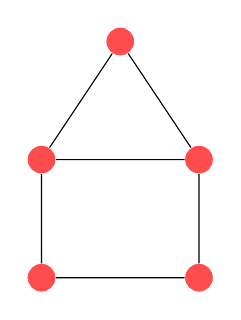
\begin{tikzpicture}[node/.style={circle,fill=red!70,minimum size=1em,inner sep=3pt]}]
       \node[node] (1) at (0, 0) {};
       \node[node] (2) at (-1, -1.5)  {};
       \node[node] (3) at (1, -1.5) {};
       \node[node] (4) at (-1, -3) {};
       \node[node] (5) at (1, -3) {};
       
       \draw (1) -- (3);
       \draw (1) -- (2) -- (4) -- (5) -- (3) -- (2);
     \end{tikzpicture}
     \caption{A undirected simple graph.}   
   \end{subfigure}
   ~
   \begin{subfigure}[t]{0.45\textwidth}
     \centering
     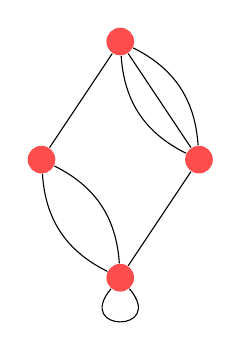
\begin{tikzpicture}[every loop/.style={}, node/.style={circle,fill=red!70,minimum size=1em,inner sep=3pt]}]
       \node[node] (1) at (0, 0) {};
       \node[node] (2) at (-1, -1.5)  {};
       \node[node] (3) at (1, -1.5) {};
       \node[node] (4) at (0, -3) {};
      
       \draw (1) -- (2);
       \draw (1) -- (3) -- (4);
       \path (2) edge [bend left] (4);
       \path (2) edge [bend right] (4);
       \path (3) edge [bend left] (1);
       \path (3) edge [bend right] (1);
       \draw (4) edge [in=-50,out=-130,loop] (4);
     \end{tikzpicture}
     \caption{A undirected graph with a self-loop and parallel edges.}
   \end{subfigure}
   
   \caption{Graphical representation of two graphs with different properties. 
   The vertices are represented by red dots and the edges are the line segments between them.} 
   \label{fig:example_graphs}
\end{figure}


The \emph{order} of a graph is its number of vertices (i.e., the cardinality of the vertex set) and is denoted as \(n = |V(G)|\). 
The neighborhood of a vertex \(v_i\) is defined as \(N(v_i) = \{v_j \in V(G) : \{v_i, v_j \} \in E(G)\}\).
It is the set of vertices that are \emph{adjacent} to the vertex \(v_i\). 
The cardinality of this set is called the \emph{degree} of the vertex and is denoted as \(d(v_i) = |N(v_i)|\). 
A vertex without any neighbors (i.e., with a degree of zero) is called \emph{isolated}.
It is also often very useful to measure degree properties for the graph. 
For example, the \emph{minimum degree} \(\delta(G) = \min\{d(v_i) : v_i \in V(G)\}\), the \emph{maximal degree} \(\Delta(G) = \max\{d(v_i) : v_i \in V(G)\}\), and the \emph{average degree} \(d(G) = \frac{1}{n} \sum_{v_i \in V(G)} d(v_i)\).
These global measures can be used to get an insight in the basic structure of the graph.

A \emph{path} on a graph can be defined as a finite sequence of vertices \(v_1,v_2,\dots,v_k\), such that between any consecutive pair of vertices exist a edge in the graph.  
Furthermore, all edges between the vertices and the vertices itself must be distinct. 
The first and the last vertices in the sequence are called the \emph{end vertices} or \emph{terminal vertices} of the path.
The \emph{path length} is the number of edges on the path.
Two vertices are \emph{connected} if it is possible to find a path with these two vertices as end points.
A vertex is, by definition, connected to itself.
If there exists a path between all pairs of vertices, then the graph is called connected.
It is possible to partition the vertex and edge set of a not connected graph in such a way that there are no edges between vertices in different partitions.
These partitions are called the \emph{components} of the graph.

The \emph{clustering coefficient} \cite{Watts1998} of a vertex is a measure for the cliquishness of its neighborhood.
A \emph{clique} in a graph is a subset of vertices, such that there exists an edge between every pair of vertices in this set.
The clustering coefficient \(C(v_i)\) is defined as the fraction of possible edges between the neighbors of the vertex \(v_i\).
There are at most \(\binom{d(v_i)}{2} = \frac{d(v_i)(d(v_i) - 1)}{2}\) possible edges between vertices in the neighborhood.
Therefore, the clustering coefficient can be calculated using the following formula.

\[ C(v_i) =  \frac{2 \, |\{\{v_j, v_k\} \in E(G) : v_j \in N(v_i) \wedge v_k \in N(v_i)\}| }{d(v_i)(d(v_i) - 1)}\]

This is, of course, a local property of one vertex.
However, it is also often useful to consider the average clustering coefficient \(C = \frac{1}{n} \sum_{v(i) \in V(G)} C(v_i)\) of the graph.
Figure \ref{fig:clustering-coefficent-examples} shows some examples for different clustering coefficients.


\begin{figure}[h]
   \centering
   \begin{subfigure}[t]{0.31\textwidth}
     \centering
     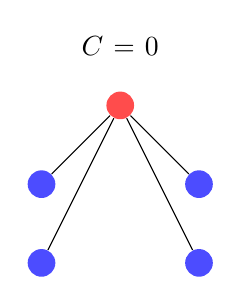
\begin{tikzpicture}[node/.style={circle,fill=red!70,minimum size=1em,inner sep=3pt]}, neighbor/.style={circle,fill=blue!70,minimum size=1em,inner sep=3pt]}]
       \node[text width=4em, align=center] at (0, 0.75)  {\(C = 0\)};
       \node[node] (1) at (0, 0) {};
       \node[neighbor] (2) at (-1, -1)  {};
       \node[neighbor] (3) at (1, -1) {};
       \node[neighbor] (4) at (-1, -2)  {};
       \node[neighbor] (5) at (1, -2) {};
       
       \foreach \p in {2,3,4,5}{\draw (\p) -- (1); }
     \end{tikzpicture}
     \caption{In this example none of the four neighbors shares a edge with any other neighbor of the red vertex.
     Therefore, the clustering coefficient of the red vertex is \(\frac{0}{6} = 0\).}   
   \end{subfigure}
   ~
   \begin{subfigure}[t]{0.31\textwidth}
     \centering
     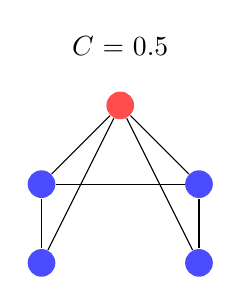
\begin{tikzpicture}[node/.style={circle,fill=red!70,minimum size=1em,inner sep=3pt]}, neighbor/.style={circle,fill=blue!70,minimum size=1em,inner sep=3pt]}]
       \node[text width=4em, align=center] at (0, 0.75)  {\(C = 0.5\)};
       \node[node] (1) at (0, 0) {};
       \node[neighbor] (2) at (-1, -1)  {};
       \node[neighbor] (3) at (1, -1) {};
       \node[neighbor] (4) at (-1, -2)  {};
       \node[neighbor] (5) at (1, -2) {};
       
       \foreach \p in {2,3,4,5}{\draw (\p) -- (1); }
       \draw (2) -- (4);
       \draw (3) -- (5);
       \draw (3) -- (2);
     \end{tikzpicture}
     \caption{Here are half of the possible edges between the neighbors are present.
     The clustering coefficient of the red vertex is \(\frac{3}{6} = \frac{1}{2}\).}
   \end{subfigure}
   ~
   \begin{subfigure}[t]{0.31\textwidth}
     \centering
     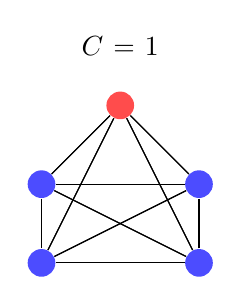
\begin{tikzpicture}[node/.style={circle,fill=red!70,minimum size=1em,inner sep=3pt]}, neighbor/.style={circle,fill=blue!70,minimum size=1em,inner sep=3pt]}]
       \node[text width=4em, align=center] at (0, 0.75)  {\(C = 1\)};
       \node[node] (1) at (0, 0) {};
       \node[neighbor] (2) at (-1, -1)  {};
       \node[neighbor] (3) at (1, -1) {};
       \node[neighbor] (4) at (-1, -2)  {};
       \node[neighbor] (5) at (1, -2) {};
       
       \foreach \p in {1,2,3,4,5}{ \foreach \q in {1,2,3,4,5}{\draw (\p) -- (\q); }}
     \end{tikzpicture}
     \caption{The neighbors of the red vertex form a clique in this example. 
     Hence, the clustering coefficient is \(\frac{6}{6} = 1\).}   
   \end{subfigure}
   
   \caption{Examples for the clustering coefficient of a vertex with a small neighborhood. 
   The blue vertices are the neighbors of the red vertex. 
   The possible number of edges between the four neighbors is \(\binom{4}{2} = 6\).} 
   \label{fig:clustering-coefficent-examples}
\end{figure}


\section{Networks and their Applications}

In the real world it is common to use graphs to model the complex systems that are arising. 
For example, the web can be represented as a graph, where the vertices correspond to websites and the edges are the hyperlinks between them. 
Another example would be a large online social networks such as Facebook, where the vertices represent the users and edges the friendship relation between them.
However, when modeling these large networks it usually common to use a slightly different terminology \cite{Barabasi2016}.
Vertices are often called \emph{nodes} and edges are called \emph{links} in the context of networks.

% TODO: large graphs = networks and network science is the statistical analysis of networks


\chapter{Model}
\label{cha:model}


The proposed user activity model with peer influence effects is in detail described in this chapter.
It is yet another extension of the activity-driven network framework by \citet{Perra2012a}, that was discussed in \cref{subsec:time-varying-network-models}.
However, it is not directly based on it, but on the work of \citet{Laurent2015}, which also relies on the the activity-driven framework.
This underlying model, which is explained in the first section of this chapter, allows for the formation of community structures and the development of strong and weak ties in the network, which is a crucial condition for the occurrence of peer influenced activity.
The additionally introduced mechanisms that allow for peer influenced activity to actually happen in the network are then discussed in \cref{sec:peer-influence-model} of this chapter.


%% ========================================================================
%% ========================================================================


\section{The Base Model}
\label{sec:base-model}


\subsection{Description}

Since this model~\cite{Laurent2015} is based on the activity-driven framework by \citet{Perra2012a}, a activity potential \( a_{i} = \eta x_{i}\),  which is drawn from a suitable distribution, is assigned to each of the \( n \) nodes.
To reflect the heterogeneous activity patterns of people, a power-law distribution \( f(x) \sim x^{-\gamma}\) is selected.
The exponent for the activity potential distribution is fixed to \( \gamma = 2.7 \), which is a value that is similar to the exponent observed in real world communication networks.
The lower bound for the activity potential is set to \( \varepsilon = 10^{-3} \), and the time scaling parameter is fixed to \( \eta = 1\), so that \( a_{i} = x_{i} \in [\varepsilon, 1] \).
Furthermore, for the sake of simplicity and without loss of generality are the size of the time window \( \Delta t \), and the number of generated links at each activation \( m \) fixed to the value \(1\) as as well.

The dynamic part of the model is basically identical to the activity-driven framework.
A node becomes active in every time window with probability equal to its activity potential and selects other nodes to interact with.
However, the goal of this model is it to produce adjustable community structures and weight-topological correlations in the integrated network, which can be archived by changing the way the communication partners are selected once a node becomes active.
More specifically, to archive these more realistic topological properties, the following two additional social mechanisms are introduced:

\begin{enumerate}
    \item Memory effects
    \item Closure processes
\end{enumerate}

The first mechanism introduces memory to the nodes, in the sense that nodes remember all previous interactions with other nodes.
This idea was adapted from the work of \citet{Karsai2014}, and enables the formation of strong ties (i.e., interactions that are repeated often) and weak ties (i.e., interactions that area repeated infrequently) between the nodes.
This heterogeneity of tie strengths is an important role for processes that take place in many real world networks.
For instance, they showed in their original paper that strong ties are able to slow down the spreading of rumors in networks of social interaction (e.g., a network of phone calls).
This counter intuitive result can be explained by the observation that most activity is concentrated and contained in strongly tied groups, which prevents a fast spreading of the rumor into other parts of the network.

The memory of a node is represented by a weighted egocentric network, that includes all other nodes that were already part of one or more interactions in the past.
These previous communication partners are also called neighbors.
The weight represents the number of previous interactions, scaled by the link-reinforcement constant \( \delta \).
\Cref{fig:egocentric-network} shows an exemplary egocentric network of the node \( v_{i} \) and its neighbors.
The choice of forming a new tie or reinforcing an existing one depends on the number of neighbors of a node.
This corresponds to the observations in social interaction dynamics, where actors tend to communicate almost exclusively within their social cycle, which has a limited size, due to cognitive capacities of the actors~\cite{Dunbar1992}.
Let \( k_{i} = d(v_{i}) \) be the degree of the node \( v_{i} \) in its egocentric network, then the probability to form a new tie is \( p(k_{i}) = \frac{c}{k_{i} + c} \), and the probability to reinforce an already established tie is \( \bar{p}(k_{i}) = 1 - p(k_{i}) = 1 - \frac{c}{k_{i} + c} = \frac{k_{i}}{k_{i} + c} \), where the constant \(c\) determines how strong the memory of an actor is (cf.  \cref{fig:reinforcement-process-prob-plot} for details).
Therefore, the probability for the formation of a new tie decays very fast with increasing size of the egocentric network.
The memory strength constant is fixed to \( c = 1 \) in the context of this work.
If an active node decides to reinforce an existing tie, the neighbor is selected proportional to the current tie strength.
Therefore, the probability for node \( v_{j} \) to be selected as communication partner of node \( v_{i} \) is given by
\( p_{i,j} = \sfrac{w_{i,j}}{\sum_{k \in N(v_{i})} w_{i, k}} \), where \( w_{i,j} \) denotes the tie strength between node \( v_{i} \) and \( v_{j} \) in the egocentric network of \( v_{i} \).
This reinforcement process allows the introduction of dependencies between successive interactions of node pairs and replaces the approach of selecting a communication partner uniformly at random when a node becomes active in the original activity-driven framework.


\begin{figure}
    \centering

    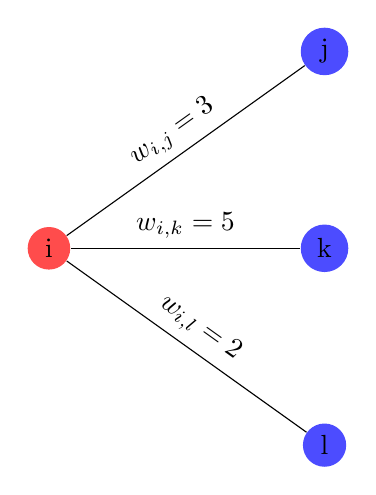
\begin{tikzpicture}[node/.style={circle,fill=red!70,minimum size=1em,inner sep=3pt]}, neighbor/.style={circle,fill=blue!70,minimum size=1em,inner sep=3pt]}]
      \node[node] (1) at (-1, -1)  {i};
      \node[neighbor] (2) at (2.5, 1.5) {j};
      \node[neighbor] (3) at (2.5, -1) {k};
      \node[neighbor] (4) at (2.5, -3.5) {l};

      \draw (1) -- (2) node [midway, above, sloped] (a) {$w_{i,j} = 3$};
      \draw (1) -- (3) node [midway, above, sloped] (b) {$w_{i,k} = 5$};
      \draw (1) -- (4) node [midway, above, sloped] (c) {$w_{i,l} = 2$};
    \end{tikzpicture}

    \caption[Egocentric network example]{Egocentric network of the node \(v_{i} \) (red node) and its neighbors \( v_{j} \), \( v_{k} \), and \( v_{l} \) (blue nodes). In this example is the link-reinforcement increment \( \delta = 1 \). This means that the weights exactly correspond to the number of previous interactions between the nodes. }
    \label{fig:egocentric-network}
\end{figure}


\myfig{reinforcement-process-prob-function}
      {width=0.75\textwidth}
      {Plots of the function that determines the probability for the formation of a new tie based on the degree of a node \( p(k) \) for different values of the memory strength \( c \). This constant can help to model different types of users. Larger values may correspond to social explorers, that are more prone to form new ties, and smaller values are related to social keepers, which communicate almost exclusively to peers in their social circle.}
      {Probability distribution for the formation of new ties.}
      {fig:reinforcement-process-prob-plot}


The second mechanism introduces two different closure processes to the model.
The first one, cyclic closure, assures the formation of triangles (i.e., cliques between three nodes), which were linked to the formation of community structures in the network by \citet{Bianconi2014}.
They showed that this mechanism is sufficient to generate networks with complex topological structures (e.g., long-tailed degree distributions), where the strength of communities depends on the cyclic closure probability.
If a node wants to form a new tie, it tries to perform a cyclic closure with probability \( p_{\Delta} \), by interacting with a randomly selected neighbor of a neighbor.
The second closure process, focal closure, tries to emulate the social dynamic that users tend to form ties with other users that are similar to them (e.g., they have common interests).
This process is performed when a new tie should be created with a probability of \( 1 - p_{\Delta} \) or if there are no suitable candidates for a cyclical closure available.
This is, for instance, the case if a node becomes active for the first time.
The weight of a new tie is always initialized to \(1\), regardless of the type of closure that was used to establish the new tie.
The actual implementation of these two closure mechanisms was adapted from the work of \citet{Kumpula2007}, who used the same closure mechanisms to study the formation of community structures in weighted static networks.
They model cyclic closure as a biased local search (cf. \cref{fig:cyclic-closure} for details) and focal closure as an unbiased global search, which means selecting a new node uniformly at random from the entire network.
Furthermore, they introduced a node deletion mechanism in their model, which was adapted here as well.


\begin{figure}
    \centering

    \begin{subfigure}[t]{0.3\textwidth}
    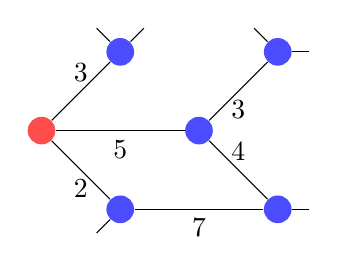
\begin{tikzpicture}[active/.style={circle,fill=red!70,minimum size=1em,inner sep=3pt]}, neighbor/.style={circle,fill=blue!70,minimum size=1em,inner sep=3pt]}]
      \node[active]   (1) at (0, 1) {};
      \node[neighbor] (2) at (1, 0) {};
      \node[neighbor] (3) at (1, 2) {};
      \node[neighbor] (4) at (2, 1) {};
      \node[neighbor] (5) at (3, 0) {};
      \node[neighbor] (6) at (3, 2) {};

      % dangling edges
      \draw (3) -- (1.3, 2.3);
      \draw (3) -- (0.7, 2.3);
      \draw (2) -- (0.7, -0.3);
      \draw (6) -- (2.7, 2.3);
      \draw (5) -- (3.4, 0);
      \draw (6) -- (3.4, 2);

      \draw (1) -- (2) node [midway, below] (a) {2};
      \draw (1) -- (3) node [midway, above] (b) {3};
      \draw (1) -- (4) node [midway, below] (c) {5};
      \draw (4) -- (6) node [midway, below] (d) {3};
      \draw (4) -- (5) node [midway, above] (e) {4};
      \draw (2) -- (5) node [midway, below] (f) {7};
    \end{tikzpicture}
    \caption{}
    \label{subfig:cyclic-closure-a}
    \end{subfigure}
    \begin{subfigure}[t]{0.3\textwidth}
    ~
    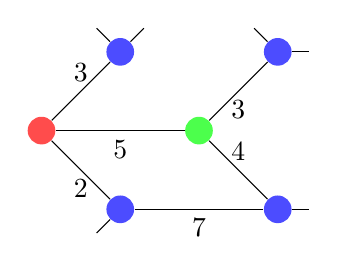
\begin{tikzpicture}[active/.style={circle,fill=red!70,minimum size=1em,inner sep=3pt]}, neighbor/.style={circle,fill=blue!70,minimum size=1em,inner sep=3pt]}, selected/.style={circle,fill=green!70,minimum size=1em,inner sep=3pt]}]
      \node[active]   (1) at (0, 1) {};
      \node[neighbor] (2) at (1, 0) {};
      \node[neighbor] (3) at (1, 2) {};
      \node[selected] (4) at (2, 1) {};
      \node[neighbor] (5) at (3, 0) {};
      \node[neighbor] (6) at (3, 2) {};

      % dangling edges
      \draw (3) -- (1.3, 2.3);
      \draw (3) -- (0.7, 2.3);
      \draw (2) -- (0.7, -0.3);
      \draw (6) -- (2.7, 2.3);
      \draw (5) -- (3.4, 0);
      \draw (6) -- (3.4, 2);

      \draw (1) -- (2) node [midway, below] (a) {2};
      \draw (1) -- (3) node [midway, above] (b) {3};
      \draw (1) -- (4) node [midway, below] (c) {5};
      \draw (4) -- (6) node [midway, below] (d) {3};
      \draw (4) -- (5) node [midway, above] (e) {4};
      \draw (2) -- (5) node [midway, below] (f) {7};
    \end{tikzpicture}
    \caption{}
    \label{subfig:cyclic-closure-b}
    \end{subfigure}
    ~
    \begin{subfigure}[t]{0.3\textwidth}
    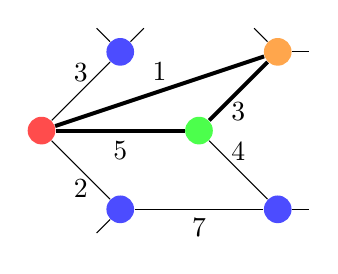
\begin{tikzpicture}[active/.style={circle,fill=red!70,minimum size=1em,inner sep=3pt]}, neighbor/.style={circle,fill=blue!70,minimum size=1em,inner sep=3pt]}, selected1/.style={circle,fill=green!70,minimum size=1em,inner sep=3pt]}, selected2/.style={circle,fill=orange!70,minimum size=1em,inner sep=3pt]}]
      \node[active]   (1) at (0, 1) {};
      \node[neighbor] (2) at (1, 0) {};
      \node[neighbor] (3) at (1, 2) {};
      \node[selected1] (4) at (2, 1) {};
      \node[neighbor] (5) at (3, 0) {};
      \node[selected2] (6) at (3, 2) {};

      % dangling edges
      \draw (3) -- (1.3, 2.3);
      \draw (3) -- (0.7, 2.3);
      \draw (2) -- (0.7, -0.3);
      \draw (6) -- (2.7, 2.3);
      \draw (5) -- (3.4, 0);
      \draw (6) -- (3.4, 2);

      \draw (1) -- (2) node [midway, below] (a) {2};
      \draw (1) -- (3) node [midway, above] (b) {3};
      \draw[line width=0.5mm] (1) -- (4) node [midway, below] (c) {5};
      \draw[line width=0.5mm] (4) -- (6) node [midway, below] (d) {3};
      \draw (4) -- (5) node [midway, above] (e) {4};
      \draw (2) -- (5) node [midway, below] (f) {7};
      \draw[line width=0.5mm] (1) -- (6) node [midway, above] (g) {1};
    \end{tikzpicture}
    \caption{}
    \label{subfig:cyclic-closure-c}
    \end{subfigure}

    \caption[Cyclic closure mechanism example]{This is an illustration of the cyclic closure mechanism in the model. The network depicted in these figures is part of the union of all egocentric networks (i.e., the integrated network). \Cref{subfig:cyclic-closure-a} shows the active node in red. In the first step, this node has to select one of his neighbors. This is done at random with respect to the tie strengths. Therefore, the probabilities for the three neighbors to be selected are \(\sfrac{3}{10}\), \(\sfrac{5}{10}\), and \(\sfrac{2}{10}\) respectively. In this example the neighbor with the highest probability was selected, which is depicted in \cref{subfig:cyclic-closure-b} (green node). Since the selected neighbor has neighbors himself that do not share a link with the active node yet, the cyclic closure can be completed. This is done once more by selecting one of the candidates at random with respect to the weight of the ties and creating a new tie with unit strength with probability \( p_{\Delta} \). \Cref{subfig:cyclic-closure-c} shows they selected node (orange node) and the newly formed triangle in the network.}
    \label{fig:cyclic-closure}
\end{figure}


In the activity-driven framework, nodes live forever and are, therefore, forever part of the network.
Here, nodes have an intrinsic probability \(p_{d}\) to be removed in every time step, which is the same for every node in the network.
This ensures that the network can reach a stable state in which the structural characteristics (e.g., the community structures) become invariant in time.
Every time a node is removed from the network, a new one joins to keep the size of the network constant.
The deletion probability of nodes can determine how fast the network reaches its equilibrium.
A small value for \(p_{d}\) allows nodes to stay a long time in the network and even nodes with relatively small activity potential can become fully integrated in the community structures.
Therefore, it takes longer to reach the time invariant state of the network when the low activity nodes are not removed fast enough.
The expected time that a node will be part of the network can be determined by viewing it as a simple Bernoulli process.
In each iteration a biased coin is tossed for every node.
The outcome of this Bernoulli random experiment determines if the nodes stays in the network or is replaced in the next round.
The probability for a node to be deleted after exactly \( x \) iterations is \( \prob{x} = (1-p_{d})^{x-1} p_{d} = \bar{p}_{d}^{x-1} p_{d}\).
Hence, the expected value for the lifetime of a node is given by \( \expval{x} = \sum_{x=1}^{\infty} x \prob{x} = \sum_{x=1}^{\infty} x \bar{p}_{d}^{x-1} p_{d} = p_{d} \sum_{x=1}^{\infty} x \bar{p}_{d}^{x-1} \).
This sum is related to the sum of the geometric series \( \sum_{x=0}^{\infty} r^{x} = \frac{1}{1 - r} \), for \(|r| < 1 \), by being its first derivative\footnote{The first derivative of the sum of the geometric series is \( \frac{\mathrm{d} \sum_{x=0}^{\infty} r^{x}}{\mathrm{d} r} = \sum_{x=0}^{\infty} \frac{\mathrm{d} r^{x}}{\mathrm{d} r} = \sum_{x=1}^{\infty} x r^{x-1} = \frac{\mathrm{d} \frac{1}{1-r}}{\mathrm{d} r} = \frac{1}{(1 - r)^{2}} \), for \(|r| < 1\).}.
Therefore, the expected value for the lifetime of a node is \( \expval{x} = \frac{p_{d}}{(1 - \bar{p}_{d})^{2}} = \frac{1}{p_{d}} \).
This means that, for example, nodes with a deletion probability of \( p_{d} = \num{5e-05} \) will be on average deleted after 20,000 iterations.


\subsection{Properties}

The properties of this model are examined by analyzing a extended version of the integrated network.
This is very similar to the basis framework, in which the temporal network is represented as a sequence of graphs.
These graphs are denoted as instantaneous networks, and the union of these networks up to a time step \( T \) is called the integrated network.
This is also true for this extension, however, the links in the integrated network have additionally a weight assigned to them, which corresponds to the tie strength in the egocentric networks of the nodes.
Another equivalent way to define the integrated network is the union of all egocentric networks up to some time step \( T \).

These newly introduced mechanisms have interesting effects on how the structures on the integrated network evolve over time.
In the beginning, after nodes form their first ties, they start to close triangles and reinforce the ties in their egocentric network.
This means that strong community structures are formed early in the process.
However, after a while more weak ties are introduced and fewer triangles are closed so that the strength of the communities declines and the network reaches its equilibrium state.
As mentioned earlier, the node deletion probability can be used to control the time until the network converges, but it can also be used to tune the strength of the communities and the average degree of the network.
A smaller value for \( p_{d} \) decreased the average local clustering coefficient and increases the average degree.

The cyclic closure probability \( p_{\Delta} \) and the reinforcement increment \( \delta \) control the formation of communities as well (see \cref{fig:community-structures-in-model}).
Furthermore, like the node deletion probability, the two parameter have an effect on the average degree of the converged network.
Higher values for the cyclic closure probability or the tie reinforcement increment result in a smaller average degree.
However, the two parameter do not influence the actual (heterogeneous) distribution of the degrees in a significant way.
The tie strengths, which are power-law distributed, are not effected by \( p_{\Delta} \), and higher values for \( \delta \) only influence the length of the tail of the distribution.
Another characteristic of this model is that the cyclic closure probability has a larger impact on the emerging community structures than the tie reinforcement increment.
This is true since \( p_{\Delta} \) effects the number of triangles directly, whereas \( \delta \) is responsible for the creation of strong ties, which increases the bias in the local search, and only assists in the process of finding suitable nodes for the triangle formation.
Additionally, the model is able to produce higher-order correlations, that are also observable in real-world networks.
For example, weight-topology correlations (i.e., stronger ties within groups) are measurable and are depended on \( p_{\Delta} \) and \( \delta \) as well.


\myfig{community-structures-model}
      {width=0.90\textwidth}
      {Depiction of the influence of \( p_{\Delta} \) and \( \delta \) on the resulting community structures (image borrowed from~\cite{Laurent2015}). The networks in the first row (a--c) were generated with a fixed value for the link reinforcement increment \(\delta = 1\) and varying values for the cyclic closure probability (from left to right: \( p_{\Delta} = 0.5 \), \( p_{\Delta} = 0.9 \), and \( p_{\Delta} = 0.995 \)). This shows that \( p_{\Delta} \) directly influences the strength of the communities. Furthermore, tie strength heterogeneities are observable, with strong ties within communities (darker link color) and weak ties between them (brighter link color).The second row shows networks with a fixed cyclic closure probability \( p_{\Delta} = 0.995 \) and different reinforcement constants (from left to right: \(\delta = 0\), \(\delta = 0.5\), and \(\delta = 1.5\)). This shows that a high probability for the formation of triangles is not enough for the formation of communities. The reinforcement process that helps to develop strong ties is required as well and also effects the size of the communities.}
      {Influence of \( p_{\Delta} \) and \( \delta \) on the community structures}
      {fig:community-structures-in-model}


%% ========================================================================
%% ========================================================================


\section{Peer Influence Extension}
\label{sec:peer-influence-model}


\subsection{Idea}

So far the activity in the temporal network was entirely determined by the activity-potential distribution.
Each node is assigned an intrinsic probability to become active in each round, which is drawn from this distribution.
The assignment is done once for every node when it gets created and does not change afterwards.
A node can become active in an iteration of the model either by himself or by being contacted by another active node.
The process of becoming active on one's own accord does not depended on whether or not the node was active in previous time steps.
This corresponds to a memory-less Poisson process and leads necessarily to exponentially distributed times between two consecutive activations of a node (i.e., inter-event times).
The significance of complex long-tailed inter-event time distributions in human behavior was already discussed in \cref{sec:user-activity-models}.
However, it is evident that activations caused by other nodes are not necessarily independent of previous events, due to the memory effects introduced in the model.
For example, lets assume a node with very low activity potential is part of group of high-activity nodes and already established strong ties.
The self-activation rate of the low-activity node will be quite low, with a mean value and standard deviation for the inter-event times that is equal to the inverse of its activity probability.
Nevertheless, the other nodes in the group will fairly often select the low-active node as communication partner when they become active, due the biased local search.
This can, of course, alter the inter-event time distributions of nodes with a small activity potential in a significant way, compared to the distributions that are generated by the activity-driven framework, where the activation through other nodes happens only at random.
This, in this case implicit, influence that nodes have on the activity on their neighbors is an interesting effect and was a starting point for this thesis.
In this section, a extension of the prior discussed base model with memory and closure effects is presented, which tries to model the influences of peers in the local network in a more explicit way.

The ideas for this model were heavily influenced by the work of \citet{Walk2016}.
They proposed a model that includes peer-influence and its impact on the state of activity in collaboration networks.
A more detailed description of their work is located in \cref{sec:peer-influence}.
The gist of the here proposed extension to the model is that a node can not only become active on its own based on its activity potential, but also by being motivated to become active by its neighbors, that were active in the previous iteration.
Another way to look at it would be that active nodes can influence their neighbors to become active as well in the next round.
Therefore, introducing a more explicit peer influence mechanism to the model.
This also means that a node now can become active in three different ways.
First, it can become active by himself either due to its intrinsic fixed activity probability or due to the influence of the nodes in its egocentric network, or it can become active in a passive way by being contact by another active node.


\subsection{Description}

The peer influence that a node \(v_{i} \) receives from its neighbors is denoted as \( p_{i} \).
Like the activity potential, \( p_{i} \) is a probability for an activation as well, but instead of being fixed, it may vary in each iteration based on the number of active neighbors in the last round.
Therefore, a more appropriate notation is \( p_{i}(t) \).
To regulate how much peer influence a node can receive at most, an upper bound \( q \) is defined, such that \( \forall t: \, 0 \leq p_{i}(t) \leq q \leq 1 \).
It denotes the maximal probability for an activation motivated by the neighbors of a node.

Since the peer influence probability depends on the neighbors that were active in the last round, the information of the last activations of the nodes must be stored.
This is done by extending the egocentric networks to save the timestamp of the last activation for each node.
The time of last activation of \( v_{i} \) is called \( t_{i} \) and is updated independent of the type of activation (i.e., due to self activation or by being contacted by another active node).
Furthermore, the peer influence probability should not only be depended on how many neighbors of a node were active in the round before, but also on the strength of the ties between them.
A neighbor that shares a strong connection with a node should be more influential than, for example, neighbors that were only recently introduced to the egocentric network.
This can easily be described by a weighted fraction of the last active neighbors.
However, to make the model more general and adaptable the following version of the weighted fraction of active neighbors at time \(t - 1\) is used, that transforms the weights beforehand.
Each weight in the egocentric networks of \( v_{i} \) is transformed and normalized by

\begin{equation}
    w'_{i,j} = \frac{\exp(\beta w_{i,j})}{\sum_{k \in N(v_{i})} \exp(\beta w_{i,k})},
\end{equation}

where \( \beta \) is a free parameter.
This corresponds to applying the softmax or normalized exponential function~\cite{Bishop2006} to each weight.
The softmax function is strongly related to the Boltzmann distribution~\cite{vanLaarhoven1987}, which describes the probability for states in a physical system (e.g., particles in a magnetic field) with respect to the systems temperature and the energy of its states.
Low energy states have a higher probability in the distribution, and as the temperature of the system gets close to zero, the probability for the state with the lowest energy is almost equal to one.
Whereas, in a high temperature system all states are nearly equiprobable.
The free parameter \( \beta \) in the softmax function is called inverse temperature and replicates this behavior.
It is defined as the reciprocal value of the temperature.
This softmax function is used in many applications in different fields besides physics as well.
For instance, it is used in the machine learning area of reinforcement learning, where the actions of agents in some setting are selected with respect to the probabilities yielded by the softmax function.
\citet{Crites1998} apply this method to control a group of elevators using multiple agents.
It is also, for example, used in the modeling of the decision making behavior of humans in economic settings~\cite{Ray2008}.


\begin{figure}
    \centering
    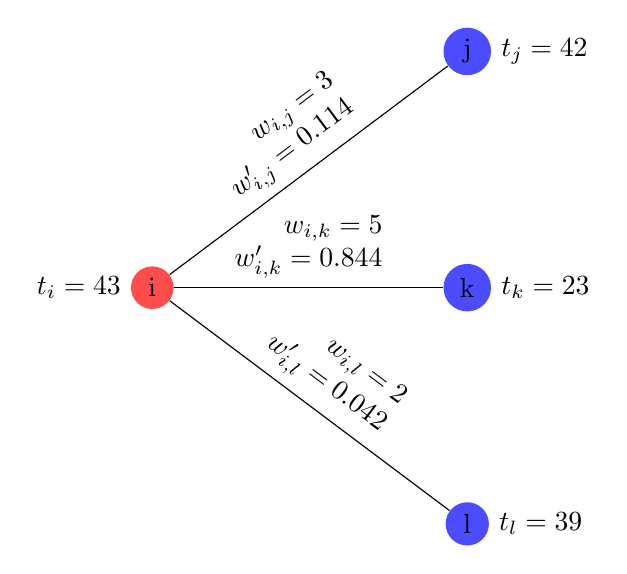
\begin{tikzpicture}[node/.style={circle,fill=red!70,minimum size=1em,inner sep=3pt]}, neighbor/.style={circle,fill=blue!70,minimum size=1em,inner sep=3pt]}]
      \node[node, label=left:{$t_{i} = 43$}] (1) at (-1, -1)  {i};
      \node[neighbor, label=right:{$t_{j} = 42$}] (2) at (3, 2.0) {j};
      \node[neighbor, label=right:{$t_{k} = 23$}] (3) at (3, -1) {k};
      \node[neighbor, label=right:{$t_{l} = 39$}] (4) at (3, -4.0) {l};

      \draw (1) -- (2) node [midway, above, sloped, align=right] (a) {$w_{i,j} = 3$ \\ $w'_{i,j} = 0.114$};
      \draw (1) -- (3) node [midway, above, sloped, align=right] (b) {$w_{i,k} = 5$ \\ $w'_{i,k} = 0.844$};
      \draw (1) -- (4) node [midway, above, sloped, align=right] (c) {$w_{i,l} = 2$ \\ $w'_{i,l} = 0.042$};
    \end{tikzpicture}

    \caption[Extended egocentric network example]{Extended egocentric network of the node \(v_{i} \) (red node) and its neighbors \( v_{j} \), \( v_{k} \), and \( v_{l} \) (blue nodes). Each node stores additionally the point in time on which it was last active. For instance, node \(v_{j} \) was last active at \( t = 42 \). Furthermore, the scaled and normalized weights \( w'_{i,j} \) are part of the network. For example, the scaled weight for the tie between \( v_{i} \) and \( v_{j} \) can be calculated by \(\sfrac{\exp(3)}{\exp(3) + \exp(5) + \exp(3)} = 0.114 \). For the sake of simplicity is \( \beta = 1 \) in this example.}
    \label{fig:extended-egocentric-network}
\end{figure}


The usage of the softmax function for this model allows different influence scenarios.
For example, a value of \( \beta = 0 \) (this would correspond to a very high temperature) would scale every weight to the same value, which means that every active neighbor influences a node equally, regardless of the tie strength.
However, it also possible to make \( \beta \) depended on the time (i.e., \( \beta(t) \)), similar to a physical system that is cooling off or heating up.
For instance, in this thesis is the temperature at time \( t \) for most experiments set to the average weight in the integrated network \( G_{T} = \sum_{i=0}^{t} G_{i}\) (i.e., \( \beta(t) = (\frac{1}{m} \sum_{(i,j) \in E(G_{T})} w_{i,j})^{-1} \)).
The normalized weights \( w'_{i,j} \) are also part of the extended egocentric (c.f. \cref{fig:extended-egocentric-network}) and must be updated at the end of every iteration.
The fraction of active neighbors \( \alpha_{i}(t) \) of node \(v_{i} \) at time \( t - 1 \) is then given by

\begin{equation}
    \alpha_{i}(t) = \frac{\sum_{j \in N(v_{i})} \mathbf{1}_{\{t_{j} = t-1\}} \exp(\beta(t) w_{i, j})}{\sum_{j \in N(v_{i})} \exp(\beta(t) w_{i, j})} = \frac{\sum_{j \in N(v_{i})} \mathbf{1}_{\{t_{j} = t-1\}} w'_{i, j}}{\sum_{j \in N(v_{i})} w'_{i, j}},
\end{equation}

where \( \mathbf{1} \) is the indicator function, which yields the value \(1\) every time the predicate is true, otherwise it is \(0\).

In the next step this weighted fraction of prior active neighbors must be mapped into a peer influence probability in the range \( [0, q] \) using a monotonically increasing function.
One possibility would be the usage of a linear function \( g(\alpha) = q \alpha \) defined for values \(0 \leq \alpha \leq 1 \).
However, this function seems to not describe the peer influence mechanism very well.
On one hand should another active neighbor not be heavily influential when there is already a large portion of neighbors active.
The peer influence should basically saturate after some fraction of neighbors is active.
On the other hand, should the peer influence for a node become noticeable after some threshold of active neighbors is reached.
This can be archived using an sigmoid function.
Similar to~\cite{Walk2016} the following algebraic sigmoid  function \( g \) is used to determine the peer influence for the node \( v_{i} \)

\begin{equation}
    p_{i}(t) = g(\alpha_{i}(t)) = \frac{\alpha_{i}(t) q}{\sqrt{\alpha_{i}^{2}(t) + \theta^2}},
\end{equation}

where the parameter \( q \) is the maximum peer influence, as discussed prior, and \( \theta > 0 \) denotes a critical threshold, which determines the required (weighted) fraction of active neighbors to set the peer influence probability close to its maximum.
Therefore, active neighbors always influence the peer influence probability, but only after a certain point in a significant way.
The satisfaction of the prior described requirements for the function can be verified by studing its first derivative \( \frac{\mathrm{d} g}{\mathrm{d} \alpha} = \frac{q \theta^{2}}{(\theta^2 + \alpha^2)^{\sfrac{3}{2}}}  \), which approaches zero very fast for values grater than \( q \).
Sigmoid functions are usually defined for all real values, since they are often used to re-scale values to the range of \([-1, 1] \) or \( [0, 1] \).
However, for this work only input values on the unit interval are relevant and the two parameter \( q \) and \( \theta \) should be selected carefully to archive the desired peer influence behavior.
For instance, too large values for \( \theta \) may obstruct the peer influence mechanism crtically, since the maximum influence may never be reached, even for \( \alpha = 1 \).
\Cref{fig:peer-influence-sigmoid} shows the discussed sigmoid function with different values for the critical threshold.


\myfig{peer-influence-sigmoid}
      {width=0.75\textwidth}
      {Depiction of the sigmoid function that is used to calculate the peer influence probability \(p_{i} \) of a node based on its (weighted) fraction of active neighbors \( \alpha \) for different values of the critical threshold \( \theta \). The maximum possible peer influence probability in this example is fixed to \( q = 0.10 \). The critical threshold determines how fast the maximum peer probability can be reached. Values in the range between 5\% and 20\% seem to be a sound choice, since already a small number of influential neighbors should suffice to have an notable effect on a user.}
      {Peer influence sigmoid function examples}
      {fig:peer-influence-sigmoid}


The process of a node becoming active by himself must be adapted as well.
The simple biased coin flip becomes a more sophisticated two-step random experiment.
First, like in the base model, a biased coin is tossed to determine if a node becomes active with probability that corresponds to its activity potential.
If this first random experiment fails the node gets a second chance to become active by himself.
This is done by calculating its peer influence probability and tossing another biased coin.
Therefore, the total probability of a node \( v_{i} \) becoming active at time \( t \) can be expressed by

\begin{equation}
    \prob{v_i \text{ becomes active}} = a_{i} + (1 - a_{i}) p_{i}.
\end{equation}

This concludes the definition of the peer influence extension of the model.
\Cref{tbl:all-model-parameter} contains an overview of all model parameter and their origin.
Note that many of them (e.g., \( \Delta t \), \( \eta \), \ldots) have reasonable default values assigned to them in the context of this work.

\begin{table}[h!]
\centering
\begin{tabular}{lp{10cm}}
\hline
\textbf{parameter} & \textbf{description} \\ \hline \hline
\multicolumn{2}{c}{activity-driven framework} \\ \hline
\( n \) & The number of nodes in the network. \\
\( f(x) \) & The probability distribution for the activity potentials of the nodes. It has a positive probability for values in the range of \( [\varepsilon, 1] \). \\
\( \varepsilon \) &  The lower bound of the activity potential. It should be \( 0 < \varepsilon \ll 1 \). \\
\( \Delta t \) &  The length of the time window in each iteration. \\
\( \eta \) &  A re-scaling factor for the activity potential to adjust the average number of active nodes in each iteration. \\
\( m \) & The number of contacts a node initiates, once it become active. \\ \hline \hline

\multicolumn{2}{c}{community structure extension} \\ \hline
\( p_{\Delta} \) & The probability to form a triangle when establishing a new tie. \\
\( p_{d} \) & The probability for node to get deleted in a iteration. \\
\( \delta \) & The constant factor that is added to the tie strength when it is reinforced. \\
\( c \) &  The memory constant, which influences the probability to form a new tie.\\ \hline \hline

\multicolumn{2}{c}{peer influence extension} \\ \hline
\( \beta \) & Inverse temperature parameter for the softmax re-scaling of the weights. This parameter may also be time depended. \\
\( q \) & The maximum possible peer influence probability that a node can receive. \\
\( \theta \) & The critical threshold for the peer influence.  \\ \hline
\end{tabular}

\caption{An overview of the parameter set of the model.}
\label{tbl:all-model-parameter}
\end{table}

\chapter{Results}
\label{cha:results}


This chapter discusses the basic findings of the analysis of the proposed peer influence model.
All results were obtained from synthetic networks, with a fixed size of \( n = 5,000 \) nodes, which were generated over \( T = 75,000 \) iterations.
The here presented properties of the time-varying networks were obtained by averaging the results of 40 independent runs, which is necessary due to the stochastic nature of the model.
The model parameter responsible for the formation of the community structures are set to \( p_{\Delta} = 0.90 \) for the triadic closure probability, \( \delta = 1 \) for the link reinforcement constant, and \( p_{d} = \num{5e-05} \) for the node deletion probability for every experiment.
Furthermore, the critical peer influence threshold was fixed to \( \theta = 0.10 \).
This reflects the idea that only a relatively small number of active neighbors is sufficient to increase the activity of a node in a significant way.

The time-dependent topological properties of the integrated network, which are discussed in \cref{sec:integrated-network-properties}, are measured only for nodes that are part of the temporal network.
This means that nodes, which were removed earlier due to the node deletion process do not influence the properties of the integrated network any more.
\Cref{sec:network-activity} contains an overview of the overall network activity with respect to different levels of peer influence.
The effect of the peer influence mechanism on the inter-event time distribution in the network is examined in \cref{sec:inter-event-time-dists}.
Furthermore, the distributions of the node degrees and tie strengths (i.e., the link weights) derived from the integrated networks are the subject of \cref{sec:weight-and-degree-distribution}.
All these experiments are performed for different values for the maximum peer influence probability \( q \).
However, the analysis performed in the last section of this chapter (\cref{sec:softmax-rescaling}) uses a fixed value for the peer influence level and discusses how different values for \( \beta \), the inverse temperature for the softmax weight rescaling, changes the peer influence effects in the network.
The temporal networks, which are used in the experiments of the first four sections of this chapter, adopt the current average tie strength as temperature for the softmax weight rescaling.
Therefore, \( \beta \) is set to the to the reciprocal value of average weight in the integrated network in each iteration after the first one (i.e., \( \beta = 1 \) in the initial round to avoid division by zero, since no ties have been formed yet).


%% ========================================================================
%% ========================================================================


\section{Time-dependent Integrated Network Properties}
\label{sec:integrated-network-properties}

Not only the final integrated network of all 75,000 instantaneous networks and its properties are of great interest, but also how they evolve during the simulation.
This allows to get a deeper understanding on how the model shapes the community structures in the network and the effects of the peer influence mechanism on it.
The integrated network is build in an iterative fashion to make these observations possible.
A snapshot of the integrated network is taken after the newly formed ties are included and the weights of already established links are updated in every time step.
Features like the average local clustering coefficient or the average weight of the ties are calculated for each of the 75,000 integrated network snapshots.
This allows to examine how the topology and other measures change over time.

The first, and most interesting, measure that can be investigated in this way is the average local clustering coefficient \( C(t) \).
\Cref{fig:avg-local-cc-full} depicts the development of it over the course of the simulation for different levels of peer influence.
The graph of this function has a very distinctive pattern, which was already explained in the original work by \citet{Laurent2015}.
The average clustering coefficient is very small in the first few hundred iterations, due to the sparsity of the integrated network.
Almost all nodes are disconnected and the number of triangles, which have already formed is relatively small compared to the size of the network.
However, \cref{fig:avg-local-cc-full} also shows that the clustering coefficient grows very fast until it reaches its maximum value after a short period of time.
This rapid increase is caused by the cyclic closure mechanism of the model.
Nodes that become active in this early stage first have to introduce some ties with nodes which are selected using the focal closure mechanism.
This does not increase the average local clustering coefficient in a significant way, however, it establishes the egocentric networks.
After the first triangles are closed, the first strong ties start to develop.
These emerging strong ties amplify the biased local search of the triadic closure mechanism and result, on one hand, in more triangles, and on the other hand, in the reinforcement of already established triangles and the associated strong ties.
This leads to a high local clustering in the established communities.
However, weak ties are eventually also introduced to the network, due to the focal closure mechanism.
They are rarely involved in the formation of new triangles, due to the bias towards strong ties, which contributes to the decrease of the average local clustering coefficient until the network reaches its stationary state.


\myfig{avg-local-cc-full}
      {width=0.75\textwidth}
      {The average local clustering coefficient \( C \) as a function of time for different maximum peer influence probabilities \( q = 0, \, 0.01, \, 0.05, \, 0.1, \, 0.15\). }
      {Average local clustering coefficient as function of time}
      {fig:avg-local-cc-full}


The peer influence mechanism seems to influence the development of the local clustering in the beginning of the simulation significantly.
\Cref{fig:avg-local-cc-start} depicts the time-dependent average local clustering coefficient in the initial phase of the simulation (i.e., for the first 10,000 iterations) for a range of possible values for \( q \).
It shows that the peak of \( C \) is reached faster for networks in which nodes are able to motivate their neighbors to some extend.
For instance, the network in which nodes are not able to influence their neighbors reaches it peak value for \( C \) after approximately 5,000 iterations, while the network with a maximum peer influence probability of \( q = 0.15 \) is more than 2,000 iterations faster.
However, the effect only occurs for networks with \( q > 0.05 \) and the actual maximum value of the local clustering coefficient only increases slightly for higher levels of peer influence (c.f. \cref{tbl:max-clustering} for the precise figures).
Furthermore, the proposed peer influence mechanism seems to have an positive effect on the development of the topological structures in the network by accelerating the process in the beginning.

The percentage of network activity, which is responsible for the reinforcement of ties in each iteration \( r(t) \) highlights this behavior as well.
In the beginning most activity is spend on the formation of new ties and therefore building the topological structures of the network, but after a while more and more activity is focused on reinforcing existing ties, which leads to a drastic increase of \( r(t) \).
This is also emphasized by the time required to reach the point from which on more than half of the total activity is spend on reinforcement.
This point is reached for the network with \( q = 0.15 \) after only 109 iterations.
The network with no peer influence takes with 229 iterations about twice as long, indicating that peer influence may play an important role in the first few iterations that shape the topology of the network.


\begin{figure}[htbp]
\centering
\begin{subfigure}[b]{0.485\textwidth}
  \includegraphics[width=\textwidth]{figures/avg-local-cc-start}
  \caption{}
  \label{fig:avg-local-cc-start}
\end{subfigure}
~
\begin{subfigure}[b]{0.485\textwidth}
  \includegraphics[width=\textwidth]{figures/avg-local-cc-end}
  \caption{}
\label{fig:avg-local-cc-end}
\end{subfigure}

\caption[Segments in the average local clustering coefficient evolution]{Segments in the evolution of the local clustering coefficient for different levels of peer influence. (\subref{fig:avg-local-cc-start}) shows the clustering coefficient for the first 10,000 iterations of the simulation, in which it reaches it maximum value and slowly starts to decrease. (\subref{fig:avg-local-cc-end}) depicts the stationary values for \( C \), which can be observed in the last 5,000 iterations.}
\label{fig:avg-local-cc-details}
\end{figure}


\begin{table}
\centering
\begin{tabular}{llllllll}
\( q \) & 0.00 & 0.01 & 0.025 & 0.05 & 0.075 & 0.10 & 0.15 \\
\midrule
\( t_{\max} \) & 5,140 & 4,919 & 4,839 & 5,192 & 4,173 & 4,044 & 3,038 \\
\midrule
\( C_{\max} \) & 0.5659 & 0.5689 & 0.5721 & 0.5773 & 0.5822 & 0.5895 & 0.5963
\end{tabular}

\caption[\( \max \) and \( \argmax \) of \( C(t) \)]{The maximum value for the local clustering coefficient \( C_{\max} = \max C(t) \) and the time to reach the maximum \( t_{\max} = \argmax C(t) \), for different values of \( q \).}
\label{tbl:max-clustering}
\end{table}


 The share of reinforcement activity does converge to a value of over 90\% for all levels of peer influence after a short period of time, which highlights the domination of the reinforcement process.
\Cref{fig:percentage-reinforced-ties} shows the plots of the percentage of reinforcement activity for the initial phase of the simulation and over all 75,000 iterations.
The plots of \( r(t) \) also reveal a link between the extent of reinforcement that is happening and the degree of peer influence.
In the network with no peer influence effects is the proportion of reinforced to created ties on average 0.8961.
The value increases to 0.9550 in the temporal network with a maximum peer influence probability of 15\%.
This can possibly be attributed to the overall increased activity within communities, due to the peer influence effects, and the associated bias towards local strong ties.
With other words, the increased local activity overshadows the introduction of random links by low-activity and/or poorly integrated nodes.


\begin{figure}[htbp]
\centering
\begin{subfigure}[b]{0.485\textwidth}
  \includegraphics[width=\textwidth]{figures/percentage-reinforced-ties-full}
  \caption{}
  \label{fig:percentage-reinforced-ties-full}
\end{subfigure}
~
\begin{subfigure}[b]{0.485\textwidth}
  \includegraphics[width=\textwidth]{figures/percentage-reinforced-ties-beginning}
  \caption{}
  \label{fig:percentage-reinforced-ties-beginning}
\end{subfigure}

\caption[Percentage of reinforced ties as function of time]{The percentage of reinforced ties \( r(t) = \sfrac{\#e_{r}(t)}{(\#e_{r}(t) + \#e_{c}(t))} \) for different levels of peer influence as a function of time, where \( \#e_{c}(t) \) and \( \#e_{r}(t) \) are the number of created ties and the number of reinforced ties in iteration \( t \), respectively. (\subref{fig:percentage-reinforced-ties-full}) shows the ratio over all 75,000 iterations and (\subref{fig:percentage-reinforced-ties-beginning}) highlights the behavior in the beginning. Both functions were smoothed using the rolling mean method to improve the quality of the plot.}
\label{fig:percentage-reinforced-ties}
\end{figure}


The evolution of the average local clustering coefficient does dependent on the node deletion probability \( p_{d} \), since low-activity nodes, which are not removed fast enough, introduce additional weak ties in the network~\cite{Laurent2015}.
However, as clearly evident in \cref{fig:avg-local-cc-full}, the possible level of peer influence does influence the clustering, and therefore the community structures of the network, as well.
The more likely an activation due to peer influence gets, the smaller the stationary value for \( C \) becomes.
\Cref{fig:avg-local-cc-end} highlights this effect well.
This can possibly be explained in a similar way as the effect caused by the deletion probability.
However, in this case not the decelerated removal of nodes is responsible for it, but the overall increase in the number of contacts between nodes.
The peer influence mechanism increases the activity in the network, especially in already formed communities (see \cref{sec:network-activity}), since active nodes motivate their neighbors to become active as well.
The probability for the formation of a new tie is inverse proportional to the size of a nodes' egocentric network.
Therefore, a active node, which is already fully integrated in its community, will reinforce one of its existing ties, or at least close a triangle, with high probability.
However, given enough tries, such a node will eventually introduce new weak ties using the focal closure mechanism as well.
Therefore, the opportunities for the introduction of random links by active nodes increases, which leads to a smaller average local clustering in general.

Two additional measures of the integrated network, the average node degree and the average tie strength, were tracked over time for different magnitudes of peer influence as well.
\Cref{fig:avg-weight-and-tie-strength} depicts the graphs for these two network properties as function of time.
Both measures show a similar general behavior.
The average degree and the average tie strength are not independent on the maximum peer influence probability in the network and do converge after the integrated network reaches its equilibrium.
The stationary values of both do increase with increasing values for \( q \) by about the same order of magnitude, which is reasonable since both measures are related to each other.
The tie strength of a node can be seen as its weighted degree.
However, the time it takes until they converge differs.
The average degree takes longer to reach its stationary value.
This can be explained by the small probability for the creation of new ties after the egocentric networks have gained a certain size.
Every new neighbor reduces the probability for the creation of new tie in the future significantly.
The average tie strength does not suffer from this problem, due to the fast development of strong ties and the decreasing probability for the introduction of weak ties. \todo{sound explanation?}
The direct effect of the peer influence mechanism on the average degree and average weight can be explained, similar to the average local clustering coefficient, by the additional activity in the temporal network.
Nodes are getting more opportunities to add additional neighbors and to strengthen their ties until they get removed.
Note that the slightly different convergence behavior of the average tie strength for the high peer influence probability \( q = 0.15 \) cannot be explained fully at this point. It may be related to the by comparison significantly slower converge of the average degree, but it is ultimately left open for possible future studies. \todo{related work}


\begin{figure}[htbp]
\centering
\begin{subfigure}[b]{0.485\textwidth}
  \includegraphics[width=\textwidth]{figures/avg-degree}
  \caption{}
  \label{fig:avg-degree}
\end{subfigure}
~
\begin{subfigure}[b]{0.485\textwidth}
  \includegraphics[width=\textwidth]{figures/avg-tie-strength}
  \caption{}
\label{fig:avg-tie-strength}
\end{subfigure}

\caption[Average degree and tie strength as function of time]{Plots of (\subref{fig:avg-degree}) the average node degree \( d(G_{T}) \) and (\subref{fig:avg-tie-strength}) the average tie strength \( \langle w \rangle \) in the network as a function of time for different maximum peer influence probabilities \( q = 0, \, 0.01, \, 0.05, \, 0.1, \, 0.15\). }
\label{fig:avg-weight-and-tie-strength}
\end{figure}


%% ========================================================================
%% ========================================================================


\section{Network Activity}
\label{sec:network-activity}


One obvious implication of the proposed peer influence mechanism is an increase in the activity in the network.
Nodes can become active by them self not only due to their intrinsic activity potential but also by the influence of their peers.
The number of nodes that become active in iteration \( t \) entirely by them self is denoted as \( \#e_{a}(t) \), and the number that becomes active motivated by others is denoted as \( \#e_{p}(t) \).
Therefore, the total number of contacts per iteration is \( \#e(t) = \#e_{a}(t) + \#e_{p}(t) \).
The number of peer influenced activations in a networks with \( q = 0 \) is trivially \( \#e_{p}(t) = 0 \), and the number of self-activations can be approximated by \( \#e_{a}(t) \approx n \expval{a_{i}} \).
For example, the approximated number of activations in a network with no peer influence effects and the prior specified parameters (\( \gamma = 2.7 \), \( \varepsilon = 0.001 \), and \( n = 5,000 \)) is \( \#e_{a}(t) \approx 12.05 \), which matches the observed figures.
In fact, this number is roughly the same for all levels of peer influence, since the process of node self-activation due to the intrinsic activity potential is independent of the peer influence mechanism.


\myfig{number-of-contacts}
      {width=0.75\textwidth}
      {Time dependent number of activations \( \#e(t) \) in the network for different levels of peer influence \( q \). The graphs were smoothed using the rolling mean method to improve the visualization.}
      {Time dependent number of activations}
      {fig:number-of-contacts}


The total number of activations, and therefore the gain in activity due to the peer influence, is depicted in \cref{fig:number-of-contacts}.
It shows that \( \#e(t) \) reaches a stationary value fast for small levels of peer influence.
However, the development of the total number of contacts per iteration is more complex for networks with a higher degree of peer influence.
The first phase can be described as a rapid increase in the number of activations, which stops after approximately 8,000 iterations.
After that the development of \( \#e(t) \) starts to relax and slow down.
It even starts to decreases slightly in the network with a maximum peer influence probability of \( q = 0.15 \).
Finally, the numbers slowly converge to their stationary values, which are reached after about 40,000 iterations.
This is also supported by the evolution of the fraction of the peer influenced contacts per iterations \( i(t) \), which shows the same general behavior (c.f. \cref{fig:percentage-peer-influenced-activity}).
This effect on the total activity in the network is possibly related to the development of the community structures and its implications on the peer influence mechanism.
The stagnation (or even reduction) of the activity begins after the maximum value for the average local clustering coefficient was reached (c.f. \cref{fig:avg-local-cc-full} for details), which is caused by the introduction of weak ties.
These new ties are possibly responsible for the merging of communities in the network, which in turn reduces the effects of the peer influence mechanism.
Inactive nodes in these newly merged communities may have a greater impact on the weighted fraction of active nodes that is required for a significant influence on nodes.
This is could especially be true for weakly integrated nodes.
However, a more detailed analysis has to be performed in the future to determine and verify the true effects, which are responsible for the observed behavior in the network activity for larger magnitudes of peer influence. \todo{future work}


\begin{figure}[htbp]
\centering
\begin{subfigure}[b]{0.485\textwidth}
  \includegraphics[width=\textwidth]{figures/percentage-influenced-activity}
 \caption{}
 \label{fig:percentage-peer-influenced-activity-full}
\end{subfigure}
~
\begin{subfigure}[b]{0.485\textwidth}
  \includegraphics[width=\textwidth]{figures/cumulative-number-of-contacts}
  \caption{}
\label{fig:percentage-peer-influenced-and-cumulative-activity}
\end{subfigure}

\caption[Percentage of peer influenced activity and cumulative activity as function of time]{Different views on the ramifications of the peer influence mechanism on the activity in the network. (\subref{fig:percentage-peer-influenced-activity-full}) depicts the evolution of the fraction of peer influenced activity \( i(t) = \sfrac{\#e_{p}(t)}{\#e(t)} \) over time for different levels of peer influence and  (\subref{fig:percentage-peer-influenced-and-cumulative-activity}) shows the aggregated number of contacts \( E(t) \) over all 75,000 iterations. The \( i(t) \) graphs were smoothed using the rolling mean method to improve the quality of the plot.}
\label{fig:percentage-peer-influenced-activity}
\end{figure}


The effects of the peer influence mechanism on the activity within the time-varying network can be observed in other ways as well.
For instance, \cref{fig:percentage-peer-influenced-and-cumulative-activity} depicts the cumulative number of contacts (i.e., \( E(t) = \sum_{i \leq t} \#e(i) \)), which highlights the quantity of additional activity that was caused by different degrees of peer influence mechanism over time.
The distribution of the number of node activations in a certain time interval is another example.
There is a shift in the bulk of the distributions, which indicates the increased probability for a larger number of activations of a node.


%% ========================================================================
%% ========================================================================


\section{Inter-event Time Distributions}
\label{sec:inter-event-time-dists}

As already mentioned in the motivation section of this thesis (\cref{sec:temporal-data}) and while discussing different ways to model user activity (\cref{sec:user-activity-models}), human activity patterns can be fairly complex.
They can be described as bursts followed by longer phases of inactivity and are usually characterized by the inter-event time distribution \( \varphi(\tau) \), which should reflect these requirements.
The inter-event times are defined, in the context of this model, as the time between two consecutive activations of a node.
The type of activation (i.e., activation due to peer influence, activity potential, or contact of another active node) is not taken into account for the here performed analysis.
Each node \( v_{i} \) in the network has its own inter-event time distribution \( \varphi_{i} \), which depends on the node's activity potential and on the influence of its peers.
However, to get a better overview on how the peer influence mechanism changes the dynamics in the network in general, the union of the inter-event time distributions of all nodes is examined.
The sequence of inter-event times is determined for every node that was active between the beginning and the end of the simulation separately and then combined into one distribution.
This distribution can be seen as a mixture of distributions~\cite{Seidel2011} of nodes, which were at some time present in the network, i.e.,

\begin{equation}
    \varphi(\tau) = \sum_{i} \pi_{i} \varphi_{i}(\tau),
\end{equation}

where \( \pi_{i} \) denotes the mixing weights, which must be selected such that \( \sum_{i} \pi_{i} = 1 \) holds.
Therefore, the mixing weights determine the importance of every individual distribution.
In this work every distribution is considered equally important and is assigned the same weight, such that the summation constraint is fulfilled.

The burstiness of human behavior is difficult to describe and even more difficult to quantify.
It is usually done using moments of the inter-event time distribution.
For instance, the coefficient of variation~\cite{Masuda2016} is defined as the ratio between the standard deviation \( \sigma \) and the mean \( \mu \) of the inter-event time distribution, i.e., \( c_{v} = \sfrac{\sigma}{\mu} \).
It takes the value \( 0 \) when the events are occurring at a fixed non-random rate.
The coefficient of variation is \( 1 \) for exponentially distributed inter-event times, which is the case for events that are generated by a Poisson process, and it can get arbitrarily large for long-tailed distributions, such as power laws.
A normalized variant of the coefficient of variation was proposed by \citet{Goh2008}, which is called burstiness parameter and is defined as

\begin{equation}
    B = \frac{c_{v} - 1}{c_{v} + 1} = \frac{\sigma - \mu}{\sigma + \mu},
\end{equation}

and takes values in the range \( -1 \leq B \leq 1 \).
It is \( B = -1 \) for regularly occurring events, \( B = 0 \) for inter-event times that originated from a Poisson process, and \( B = 1 \) for a distribution that was derived from a extremely bursty sequence of events.
A nice property of this measure is that it can also be applied to mixture distributions that contain the inter-event times of, for example people, with different intrinsic activity levels.
For instance, the inter-event times of power-users that use a system heavily every day can be combined with those of users that use it only irregularly and the burstiness parameter is able to capture the level of burstiness that is present in the usage of the system regardless.
Therefore, it is also applicable for the inter-event time distributions derived from the simulations of the peer influence model.
The burstiness parameter for a network with no peer influence is about \( B = 0.19 \).
The introduction of peer influence increases this value, however, a drastic increase can only be observed for a maximum peer influence probability of \( q \ge 0.15 \).
\Cref{tbl:burstiness-parameter} contains the mean, standard derivation and burstiness parameter of the inter-event time distribution for a maximum peer influence probability in the range \( 0 \leq q \leq 0.15 \).


\begin{table}
\centering
\begin{tabular}{llllllll}
\( q \) & 0.00 & 0.01 & 0.025 & 0.05 & 0.075 & 0.10 & 0.15 \\
\midrule
\( \mu \) & 198.71 & 184.59 & 164.26 & 132.80 & 102.43 & 76.28 & 37.23 \\
\midrule
\( \sigma \) & 291.32 & 270.49 & 241.40 & 197.38 & 155.09 & 118.04 & 61.22 \\
\midrule
\( B \) & 0.1890 & 0.1888 & 0.1902 & 0.1956 & 0.2045 & 0.2149 & 0.2437
\end{tabular}

\caption[Burstiness of inter-event time distributions]{Mean value, standard deviation and the resulting burstiness parameter of the inter-event time distribution for different levels of peer influence.}
\label{tbl:burstiness-parameter}
\end{table}


This indicates that the peer influence mechanism influences the burstiness of the node activations.
In a network with no peer influence are two consecutive self-activations independent of each other.
Therefore, the activations happen at a certain rate that is proportional to the activity potential of a node, which leads to exponentially distributed inter-event times~\cite{Moinet2016}.
This should lead to a burstiness parameter that is close to \( B = 0 \).
However, this is not the case for the inter-event times that were generated with the proposed model even though peer influence was disabled (c.f. \cref{tbl:burstiness-parameter}).
It can be explained by the memory effects in the model, which allow reoccurring interactions within groups of nodes and by the inclusion of passive activations due to other active nodes in the calculation of the inter-event times.
A node with a higher intrinsic activity potential will select a node from its local group with high probability.
Hence, this more active node activates less active nodes regularly, which can lead to a more bursty looking activity pattern for the other nodes and explains (at least partially) the burstiness value of \( B = 0.19 \).
The peer influence mechanism of this model should amplify this effect even further, since it increases the activity within communities.
Furthermore, the activation of nodes possibly triggers cascading activations within the communities, which makes bursts more likely as well.


\myfig{inter-event-time-dist-loglog}
      {width=0.75\textwidth}
      {Log-log Plot of the inter-event time distribution for different maximum peer influence probabilities \( q = 0, \, 0.01, \, 0.05, \, 0.1, \, 0.15\).}
      {Log-log plot of the inter-event time distribution}
      {fig:inter-event-time-dist-loglog}


\myfig{inter-event-time-dist-start}
      {width=0.75\textwidth}
      {Plot of the bulk of the inter-event time distribution for small inter-event times in the range \( 1 \leq \tau \leq 10 \) for different levels of peer influence.}
      {Bulk of the inter-event time distribution}
      {fig:inter-event-time-dist-start}


One way to examine how the peer influence mechanism changes the inter-node-activation times in the network is to inspect their distribution visually.
\Cref{fig:inter-event-time-dist-loglog} depicts the inter-event distributions for a variety of peer influence levels.
The plot shows the distribution on a log-log graph, where both axis are scaled logarithmically.
This highlights that longer inter-event times are indeed possible between two consecutive activations.
The plot also shows that the level of peer influence in the network changes the shape of the distribution.
Smaller inter-event times become more likely for higher levels of peer influence, which can also be seen in the change in the mean of the distributions (c.f. \cref{tbl:burstiness-parameter}).
The average time between activations decreases from about 200 in a network with no peer influence at all, to 38 in a network with \( q = 0.15 \).
The changes in the distribution is even more noticeably for inter-event times less than ten time steps.
\Cref{fig:inter-event-time-dist-start} depicts the distributions for this interval of \( \tau \).
The probability for two successive activations increases drastically from less than 2\% to almost 22\% over the range of possible values for \( q \).
This development of the probabilities possibly explains the increase of the burstiness of the distributions, since a larger number of events within a small time frame becomes more probable due to the peer influence mechanism.
However, the tail of the inter-event time distribution changes for higher levels of peer influence as well.
Large inter-event times become more and more unlikely for larger values of \( q \), and the length of the tail decreases as well.
The values for the standard derivation of the distributions reflect this behavior as well (c.f. \cref{tbl:burstiness-parameter}).
The standard derivation of the inter-event times in the network with high peer influence effects is only about one fifth of the standard derivation in the network without peer effects.
This, of course, prevents longer intervals of inactivity to a certain extend, which is the second crucial requirement for realistic activity patterns.


%% ========================================================================
%% ========================================================================


\section{Degree and Tie Strength Distribution}
\label{sec:weight-and-degree-distribution}

While \cref{sec:integrated-network-properties} examines the average degree and tie strength as a function of time, are the distributions of these two properties the topic of discussion in this section.
Both distributions are obtained from the extended version of the integrated network, which contains all nodes that were present in the last iteration of the simulation.
The degrees and tie strengths of nodes that were deleted in previous iterations are not part of the results.
The ramifications of the closure mechanisms and the memory process on the distributions were already a subject in the original work by \citet{Laurent2015}.
They showed that both the degrees and the tie strengths are heterogeneously distributed.
Furthermore, the shape of the degree distribution is only slightly effected by the triadic closure probability \( p_{\Delta} \) and the tie reinforcement increment \( \delta \).
However, while not being effected by \( p_{\Delta} \), the tie strength distribution does dependent on the memory process of the model.
For instance, larger values for \( \delta \) increase the length of the tail.
Nevertheless, a more important issue are the effects on the degree and tie strength distributions by the proposed peer influence mechanism.

First and most important, the peer influence mechanism does not effect the heterogeneous nature of both distributions, which is an often observed property in many real world networks~\cite{Barabasi2002, Karsai2014}.
The resulting possibilities for nodes with higher degree indicate the presence of hubs, which may play, depending on the context, various important roles in networks.
\Cref{fig:degree-dist} depicts the right-skewed degree distributions for networks with different levels of peer influence.
It shows that not only the average degree in the network is directly effected by the peer influence process, but the distribution itself as well.
Nodes with small degrees become less probable, while higher degree nodes become more frequent with the increasing magnitude of peer influence.
However, the tail of the distribution does not seem to be significantly effected by the process.
The change in the shape of the distribution is in line with the already observed increasing average degree and can be explained by the same argument as well.
The boost in node activations caused by the influence of the neighbors leads to more opportunities for the formation of new ties and consequently to larger egocentric networks.


\myfig{degree-distribution}
      {width=0.75\textwidth}
      {Depiction of a degree distribution of the integrated network for different maximum peer influence probabilities \( q = 0, \, 0.01, \, 0.05, \, 0.1, \, 0.15\).}
      {Degree distribution}
      {fig:degree-dist}


\myfig{weights-distribution}
      {width=0.75\textwidth}
      {Log-log plot of the distribution of the tie strengths (i.e., the link weights) in the integrated network for different degrees of peer influence.}
      {Tie strength distribution}
      {fig:weights-dist}

The memory process is primary responsible for the heterogeneous tie strength distribution and the introduction of the peer influence mechanism does in fact not change the distribution in a significant way.
\Cref{fig:weights-dist} shows the distributions for different values for the maximum peer influence probability.
It could be expected that the increased activity within the temporal network would extend the tail of the distribution, however, this is not the case.
A possible explanation of this effect is related to the increased average size of the egocentric networks.
More neighbors imply a larger number of strong ties as well, which require frequent contacts to develop.
Therefore, the additional activations caused by the peer influence mechanism are spend on the development of the additional strong ties and not reinforcing the existing ones, which would enlarge the tail.
This would also explain the more frequent weights in the lower double-digit region, which is a consequence of the on average increased tie strength for networks with peer effects.


%% ========================================================================
%% ========================================================================


\section{Tie Strength Rescaling Scenarios}
\label{sec:softmax-rescaling}

Nodes are only able to influence their peers if they were active in the previous iteration.
The magnitude of influence does depend on the strength of the ties between nodes.
This is based on the idea that the activity of a close friend should be more effective to motivate a person to become active as well than the activities of acquaintances.
The weights (i.e., the strength of the ties) are usually rescaled in such a way that larger weights become even larger to amplify the importance of close neighbors.
This can be archived using the softmax function, which also allows to control the weight rescaling process even more using the inverse temperature parameter \( \beta \).
This free parameter can vary in time as well to allow for different rescaling characteristics depending on the progress of the simulation.
Furthermore, it also allows for various peer influence scenarios, in which nodes get influenced in different extents depending on the situation.
This section highlights the ramification on the peer influence mechanism for the following three different weight rescaling strategies.
Note that the results for the scenarios are obtained from synthetic networks with a fixed maximum peer influence probability of \( q = 0.05 \).
All other model parameter are set to the same values that are used in the other experiments as well.

\myparagraph{\( \beta(t) = \langle w \rangle (t)^{-1} \)}
The temperature for the softmax rescaling is set to the average tie strength in the snapshot of integrated network at time \( t \).
This scenario is used for all other previously discussed experiments in this chapter.
\Cref{sec:integrated-network-properties} shows that the average tie strength does increase over time until it reaches its stationary value.
Therefore, this effectively introduces a bias towards stronger ties in the early stages of the simulation that decays over time.
The activity of close neighbors influences nodes in a larger extent in the beginning, which is possibly beneficial for the formation of the community structures.

\myparagraph{\( \beta(t) = 1 \)}
In this scenario the inverse temperature parameter is fixed to the constant value \( 1 \) for each iteration.
Therefore, the bias towards strong ties is overall more prominent compared to the previous scenario and does not change during the entire simulation.
This may lead to situations in which only a very small number of neighbors do actually influence a node once they become active, since weaker ties with other nodes become so insignificant that they do not exercise considerable influence anymore.
Hence, only one of the highly influential neighbors is possibly enough to influence a node at the maximum possible level.

\myparagraph{\( \beta(t) = 0 \)}
In the last scenario \( \beta \) is fixed to \( 0 \), which basically disables the softmax weight rescaling entirely and assigns each tie the exact same weight.
The strength of the tie between any ordered pair of nodes \( (v_{i}, v_{j}) \) in the network is set to \( w'_{i,j} = \sfrac{1}{|N(v_{i})|} \).
This allows neighbors, which share a weak tie with a node to exercise the same degree of peer influence as strong tied neighbors.
Therefore, an on average larger number of active neighbors may be required to reach the maximum possible magnitude of peer influence for a node.

It seems reasonable to examine the change in the network activity for the three different rescaling scenarios, since most of the explanations for the effects observed in the other experiments are related to it.
\Cref{fig:activity-beta-scenarios} shows the number of interactions between nodes and the fraction of peer influenced interactions as function of time for the three different scenarios.
Compared to the rescaling scenario that adapts to the average tie strength in the network, an overall decrease in the number of interactions is observable in the \( \beta = 1 \) scenario.
This behavior can be attributed to an excessive bias towards strong ties.
Nodes only become active by them self due to their intrinsic activity potential or possibly if one or two of their strong tied neighbors were active in the round before.
This possibly restricts possible cascading activations within groups as well, since weakly tied nodes are node able to propagate activations properly.
The number of contacts and the fraction of those activations that were peer influenced increase rapidly in the first few hundred iterations in the \( \beta = 1 \) scenario and decreases slightly after they reached their maximum value.
This small decrease is not observable in the other two scenarios and can possibly be attributed to the weight heterogeneity that starts to emerge at this point in time in the network, which amplifies the effect.


\begin{figure}[htbp]
\centering
\begin{subfigure}[b]{0.485\textwidth}
  \includegraphics[width=\textwidth]{figures/number-of-contacts-beta}
  \caption{}
  \label{fig:number-of-contacts-beta}
\end{subfigure}
~
\begin{subfigure}[b]{0.485\textwidth}
  \includegraphics[width=\textwidth]{figures/percentage-influenced-activity-beta}
  \caption{}
\label{fig:percentage-influenced-activity-beta}
\end{subfigure}

\caption[Network activity with different rescaling scenarios]{Depiction of the influence on the activity over time for different values of \( \beta \), the inverse temperature for softmax rescaling. (\subref{fig:number-of-contacts-beta}) shows the number of interactions for each iteration \( \#e(t) \) and (\subref{fig:percentage-influenced-activity-beta}) depicts the fraction of activations that were caused by the peer influence mechanism \( i(t) \). The graphs were smoothed using the rolling mean method to improve the quality of the visualization.}
\label{fig:activity-beta-scenarios}
\end{figure}


The scenario that disables the softmax weight rescaling using \( \beta = 0 \), however, does increase the number of contacts in the network in each iteration drastically.
The expected larger number of active neighbors, which is required to motivate a node seems to be archived fairly often.
This can possibly attributed to the relatively low critical peer influence threshold \( \theta = 0.10 \), which should probably be adjusted for this rescaling scenario.
Furthermore, the network activity does not convergence in this scenario.
One possible explanation for the continuous increase in the number of contacts could be attributed to self-enhancing cascading activation effects going through the network.
However, this requires additional investigation and is a possible topic for future studies. \todo{future work}

\chapter{Conclusion}
\label{cha:conclusion}

This last chapter of the thesis not only presents a review on the achieved results, but also includes a short summary of the preceding chapters.
It contains a discussion of possible limitations of the proposed peer influence model and the methods that were used for its evaluation.
The chapter concludes with suggestions for possible future studies.
These suggestion include improvements for the model itself, and potential interesting experiments on synthetic and real-world networks.


%% ========================================================================
%% ========================================================================


\section{Recap}
\label{sec:recap}

We start our work with a brief motivational section, which sequentially leads to the incentive for the proposal of an extension to the activity-driven time-varying network framework~\cite{Perra2012a}, which incorporates peer influence effects.
The key idea behind the proposal is that people do not solely perform actions based on their intrinsic motivation, but also because of the influence of their peers.
This idea stands in contrast to the activity-driven network model, in which nodes can become active only by them self based on their activity potential.
Therefore, it provides an ideal foundation to implement a model with a peer influence mechanism on top of it.

Moreover, preliminaries on the basic topics of graph theory, various types of networks and related generative models, and time-varying networks are discussed.
These are essential for the subsequent definition and evaluation of the proposed model.
A detailed review on the activity-driven framework itself, the properties of the temporal networks it generates, and on the latest related literature that either adapts or extents it, is performed as well.
Furthermore, an overview on sociological peer influence studies and network models, which utilize different types of peer influence mechanisms, is also an element of our work, to highlight the rationale behind the proposed model.

The presence of peer influence effects requires social structures, such as tie strength heterogeneities and community structures, to exist in the network and while the basic activity-driven framework is capable of generating rich topological structures, it is not able to provide these preconditions.
To overcome this issue, an extension of the framework by \citet{Laurent2015} is utilized as actual foundation for the proposed model.
It introduces memory effects and closure processes to allow for the formation of communities and weight-topological correlations in the temporal network.
The mechanisms and properties of this model are discussed in detail as well, followed by the comprehensive definition of the peer influence extension, which was heavily influenced by the work of \citet{Walk2016}.

The actual specification of the peer influence mechanism resolves various important issues such as,

\begin{itemize}[\itemsep=\parsep]
    \item how to quantify the influence of neighbors in the egocentric network of a node,
    \item how to determine the relative influence of individual neighbors based on the tie strengths, or
    \item what additional components must be included into the model to store the for the peer influence mechanism relevant information.
\end{itemize}

After the model\footnote{An open-source implementation of the proposed model can be found at \url{https://github.com/dumfug/PIModel}} was fully specified, we evaluated it on synthetic networks.
This included an examination of the effects on the topological structures of the network, which showed that the peer influence mechanism does accelerate the formation of the community structures and influences their strength.
Additional investigations on the increased activity within the network and its implications was conducted as well.
They revealed not only the complex behavior of the activations per iteration over time for larger magnitudes of peer influence, but also the impact on the activation patterns of nodes.
The distribution of time intervals between two consecutive activations changed in a way that allows for increased burstiness, which is a property that is observable in human activity patterns.
Finally, we performed an evaluation of three different scenarios that vary the relative influence of the tie strengths between nodes and their effects on the overall network activity.
This revealed interesting consequences, especially in the case in which the influence of nodes was set to be independent of the actual tie strengths, which resulted in diverging levels of activity in the network.


%% ========================================================================
%% ========================================================================


\section{Limitations}
\label{sec:limitations}

One shortcoming, which effects all performed experiments, is the relatively small size of the generated networks.
The number of nodes in many real-world networks can be multiple orders of magnitude larger.
However, to simulate temporal networks of this size efficiently, improvements in implementation of the model must be made, which minimize the additional overhead of the peer influence mechanism.
Nevertheless, this would possibly help to explain some observed effects better.
For example, the temporarily decrease in the network activity for higher levels of peer influence, which could possibly be explained by the merging of communities in the network, is probably more prominent in larger networks.

Simulations of the model with an increased number of nodes would also allow to compare the properties of synthetically generated networks with those of real-world data sets more easily and therefore, help to verify the validity of the proposed model.
This would not only be highly interesting for topological features like clustering, but also the inter-event time distribution.
The observed changes in the distribution do not fully capture the discussed characteristics of human activity patterns, which are bursts followed by longer intervals of inactivity.
While the probability for short breaks between activation increases with additional peer influence, which matches the first requirement, declines the length of the tail.
This, again, restricts the possibilities for longer intervals between bursts.

A possible explanation for this behavior is the imbalance of the peer influence mechanism.
On one hand does a level of peer influence, which is set too low, not affect the activity significantly, on the other hand becomes the process too dominant for higher levels and leads to bursts within communities that are repeated over and over again.
A potential solution would be to restrict the peer influence process in a way that nodes cannot be easily influenced multiple times within a short period of time (i.e., a cool down time of the effect).
However, this requires additional investigation on how these cascading peer influence effects work.


%% ========================================================================
%% ========================================================================


\section{Future Work}
\label{sec:future-work}

The proposed peer influence model provides various opportunities for possible extensions and experiments.
The following examples should give some thought-provoking impulses.

\paragraph{Dynamic Processes}
A common use case of time-varying networks is their ability to study dynamic systems~\cite{Holme2015} in great detail.
Two common types of these dynamic processes are epidemic models and opinion spreading models.
The first one deals with the spreading of diseases.
It typically consists of a set of states (e.g., susceptible, infected, recovered,\ldots), which nodes can adopt, and transition rules between them.
Such models can, for example, be used to study disease containment strategies.
Opinion spreading models on the other hand deal with the spreading or adaption of certain concepts (e.g., opinions, ideas, products,\ldots), which usually have different spreading mechanisms.
The in this thesis proposed model could be used as a framework to study such dynamic processes with respect to peer influence effects.

\paragraph{Negative Peer Influence}
Peer influence is always considered a positive force in the current version of the proposed model, which changes the activity level of nodes in a positive way.
This could, for example, be observable in the context of open source projects in which the activity of maintainers increases the motivation of others to contribute as well.
However, the activity of people in some social scenarios may lead to the opposite effect too.
For example, a large number of malicious contributions (e.g., due to trolls) in online communities may induce an decline in the overall interest in the website.
Therefore, it would be also feasible to introduce negative peer effects in the model, which reduces the activity of nodes, and study its implications.

\paragraph{Peer Influence Mechanics}
The way the peer influence mechanism was implemented in the proposed model was heavily based on the work by \citet{Walk2016} and on the intuitive understanding of the concept.
However, no claim to completeness and correctness for the presented model is made.
There is always potential for improvement by the inclusion of new ideas or the removal of existing elements of the model.
For example, the complex softmax weight rescaling mechanism could be replaced with a simple weighted fraction.
This would remove one free parameter and possibly improve the runtime performance.
Another possible extension would be the introduction of a critical peer influence threshold, which depends on the size of the egocentric network of a node.
This would allow for additional peer influence scenarios, like reduced influence for hubs.


\appendix                       %% closes main document, appendix follows until end; only available in book-classes
\addpart*{Appendix}             %% adding Appendix to tableofcontents

\chapter{Power-law Probability Distribution}


In this thesis we often refer to power-law probability distributions, especially in the context of activity-driven models.
However, for the sake of simplicity the exact formula of the distribution is never explicitly stated.
This appendix contains the derivation for the exact density, distribution function, and the mean value of the probability distribution.
Additionally, it contains an example and a short description of the inverse transform sampling method, which is used in the implementation of the model.
However, all this requires a more formal definition of the distribution, so let \( X \) be a continuous random variable with the probability density function \( f(x) \sim x^{-\gamma} \), taking values in the range \( X \in [\epsilon, 1] \), with \( \gamma > 0 \) and \( 0 < \varepsilon \leq 1 \).


%% ========================================================================
%% ========================================================================


\section{Probability Density Function}
\label{sec:pdf}

The probability density function (PDF) of the power-law distributed random variable \(X\), which is defined above, is stated in a more detailed form in \cref{eq:pdf}.

\begin{equation}
	f(x) =
	\begin{cases}
		c x^{-\gamma} & \varepsilon \leq x \leq 1 \\
		0             & \text{otherwise.}
	\end{cases}
\label{eq:pdf}
\end{equation}

The factor \( c \) denotes a normalizing constant, which ensures that the function fulfills the properties of a probability density function (i.e., \( \int_{-\infty}^{\infty} f(x) \, \mathrm{d}x = 1 \)).
To calculate the normalizing constant, \cref{eq:pdf} must be solved for \( c \), i.e.,

\begin{align}
\begin{split}
	& \int_{-\infty}^{\infty} cx^{-\gamma} \, \mathrm{d}x = c \int_{\varepsilon}^{1} x^{-\gamma} \, \mathrm{d}x = c \, \frac{x^{1-\gamma}}{1-\gamma}  \bigg |_{\varepsilon}^{1} = c \, \frac{1 - \varepsilon^{1-\gamma}}{1-\gamma} = 1 \\
	& \Leftrightarrow \, c = \frac{1-\gamma}{1 - \varepsilon^{1-\gamma}}.
\end{split}
\label{eq:normalizing-const}
\end{align}


%% ========================================================================
%% ========================================================================


\section{Cumulative Distribution Function}
\label{sec:cdf}

The cumulative distribution function (CDF) is used to calculate the probability that a random variable with a probability distribution \( f \) takes a value less than \( x \), i.e.,

\begin{equation}
	\prob{X \leq x} = F(x) = \int_{-\infty}^{x} f(t) \, \mathrm{d}t.
\label{eq:cdf-def}
\end{equation}

The derivation of the cumulative distribution function for the power-law distribution defined above is done in \cref{eq:cdf}.
Note that this result only holds for values of \( \gamma \neq 1 \).

\begin{equation}
	F(x) = \int_{-\infty}^{x} ct^{-\gamma} \, \mathrm{d}t = c \, \frac{t^{1-\gamma}}{1-\gamma}  \bigg |_{\varepsilon}^{x} = \frac{c}{1-\gamma} \Big( x^{1 - \gamma} - \varepsilon^{1 - \gamma} \Big)
\label{eq:cdf}
\end{equation}

Due to the range of possible values that can be taken by the probability density with positive probability, the CDF can be rewritten as a piece-wise function, i.e.,

\begin{equation}
	F(x) =
	\begin{cases}
		0 & x < \varepsilon \\
		\frac{c}{1-\gamma} \Big( x^{1 - \gamma} - \varepsilon^{1 - \gamma} \Big) & \varepsilon \leq x < 1 \\
		1 & x \geq 1
	\end{cases}
\label{eq:cdf-pieces}
\end{equation}


%% ========================================================================
%% ========================================================================


\section{Expected Value}
\label{sec:expected-value}

The expected value of the random variable \( X \), which was defined in the beginning, is derived as follows,

\begin{align}
\begin{split}
	\expval{X} & = \int_{-\infty}^{\infty} x f(x) \, \mathrm{d}x = \int_{\varepsilon}^{1} x f(x) \, \mathrm{d}x = c \int_{\varepsilon}^{1} x x^{-\gamma} \, \mathrm{d}x \\
	    & = c \int_{\varepsilon}^{1} x^{-\gamma+1} \, \mathrm{d}x = c \frac{x^{2-\gamma}}{2-\gamma}  \bigg |_{\varepsilon}^{1} = \frac{c}{2-\gamma} \Big(1 - \varepsilon^{2-\gamma}\Big)
\end{split}
\label{eq:exp-val}
\end{align}


%% ========================================================================
%% ========================================================================


\section{Example: \( \gamma = 2.5 \) and \( \varepsilon = 10^{-2} \)}
\label{sec:example}

For this example, the exponent parameter of the distribution is set to \( \gamma = 2.5 \) and the lower bound is fixed to \( \varepsilon = 0.01 \).
These parameter require a normalizing constant of \( c = \sfrac{1}{666} \).
Therefore, the density is \( f(x) = \sfrac{x^{-2.5}}{666} \) and has a expected value of \( 0.027 \).
\Cref{fig:example-pdf} and \cref{fig:example-cdf} show the plots for the probability distribution function and the cumulative distribution function for this example, respectively.

\myfig{example-pdf}
      {width=0.75\textwidth}
      {Log-log plot of the probability density function \( f(x) = \frac{x^{-2.5}}{666 }\) taking values in the range \( [0.01, 1] \).}
      {Example probability density function of a power-law distribution.}
      {fig:example-pdf}

\myfig{example-cdf}
      {width=0.75\textwidth}
      {Plot of the cumulative distribution function of the power-law distribution described by the PDF \( f(x) = \frac{x^{-2.5}}{666} \) taking values in the range \( [0.01, 1] \).}
      {Example cumulative distribution function of a power-law distribution.}
      {fig:example-cdf}


%% ========================================================================
%% ========================================================================


\section{Inverse Transform Sampling}
\label{sec:inverse-transform-sampling}

To generate samples from the prior defined power-law distribution, the inverse transform sampling method is used in the context of this thesis.
This algorithm is based on the inversion principle~\cite{Devroye1986}.
It states that if \( U \) is a uniform random variable on the unit interval (i.e., \( U \sim \mathcal{U}(0,1) \)), then the random variable \( Y = F^{-1}(U) \) has the probability distribution function \( F \), where \( F^{-1} \) is the inverse distribution function.
The proof of this theorem is very short (cf. \cref{eq:proof-inversion-principle}) and exploits the fact that \( \prob{U \leq x} = x \) for a random variable \( U \sim \mathcal{U}(0,1) \).

\begin{equation}
    \prob{Y \leq x} = \prob{F^{-1}(U) \leq x} = \prob{U \leq F(x)} = F(x)
\label{eq:proof-inversion-principle}
\end{equation}

The actual algorithm is very short and simple as well.
To draw a sample from a distribution with a cumulative distribution function \( F \), execute the following two steps:

\begin{enumerate}
    \item Draw a number \( r \) uniformly at random from the unit interval \( [0, 1] \).
    \item Calculate \( F^{-1}(r) \) to obtain the sample.
\end{enumerate}

However, the inverse transform sampling method requires the inverse of the cumulative distribution function \( F^{-1} \).
This can, for example, be done by solving \( F(x) = y \) for \( x \).
The inverse CDF for the power-law distribution is

\begin{equation}
    F^{-1}(x) = \Big( \frac{x(1-\gamma)}{c} + \varepsilon^{1-\gamma} \Big)^{1/1-\gamma}.
\end{equation}

See \cref{eq:inverese-cdf} for the derivation.
\Cref{fig:example-sampled-pdf} depicts an approximation of a power-law distribution that was generated using the inverse transform sampling algorithm.

\begin{align}
\begin{split}
	\frac{c}{1-\gamma} \Big( x^{1 - \gamma} - \varepsilon^{1 - \gamma} \Big) & = y \\
    x^{1-\gamma} - \varepsilon^{1-\gamma} & = \frac{y(1-\gamma)}{c} \\
    x^{1-\gamma} & = \frac{y(1-\gamma)}{c} + \varepsilon^{1-\gamma} \\
    x & = \Big( \frac{y(1-\gamma)}{c} + \varepsilon^{1-\gamma} \Big)^{1/1-\gamma}
\end{split}
\label{eq:inverese-cdf}
\end{align}


\myfig{example-sampled-pdf}
      {width=0.75\textwidth}
      {The estimated probability density function of \(f(x) = \frac{x^{-2.5}}{666}\), taking values in the range \([0.01, 1]\) (i.e., the PDF from the example in \cref{sec:example}). The approximation is archived using \(n = 5000\) samples, obtained using the inverse transform sampling method.}
      {Inverse transform sampling example.}
      {fig:example-sampled-pdf}


\printbibliography


%%%% end{document}
\end{document}
